\documentclass[a4paper]{article}

\usepackage[pdftex,
  hidelinks,
  pdfauthor={Dexter Chua},
  pdfsubject={Cambridge Maths Notes: Part IB - Optimisation},
  pdftitle={Part IB - Optimisation},
pdfkeywords={Cambridge Mathematics Maths Math IB Easter Optimisation}]{hyperref}

\title{Part IB - Optimisation}
\author{Lectured by F. A. Fischer\\\small Notes taken by Dexter Chua}
\date{Easter 2015}

% Imports
\ifx \nextra \undefined
  \usepackage[pdftex,
    hidelinks,
    pdfauthor={Dexter Chua},
    pdfsubject={Cambridge Maths Notes: Part \npart\ - \ncourse},
    pdftitle={Part \npart\ - \ncourse},
  pdfkeywords={Cambridge Mathematics Maths Math \npart\ \nterm\ \nyear\ \ncourse}]{hyperref}
  \title{Part \npart\ - \ncourse}
\else
  \usepackage[pdftex,
    hidelinks,
    pdfauthor={Dexter Chua},
    pdfsubject={Cambridge Maths Notes: Part \npart\ - \ncourse\ (\nextra)},
    pdftitle={Part \npart\ - \ncourse\ (\nextra)},
  pdfkeywords={Cambridge Mathematics Maths Math \npart\ \nterm\ \nyear\ \ncourse\ \nextra}]{hyperref}

  \title{Part \npart\ - \ncourse \\ {\Large \nextra}}
\fi

\author{Lectured by \nlecturer \\\small Notes taken by Dexter Chua}
\date{\nterm\ \nyear}

\usepackage{alltt}
\usepackage{amsfonts}
\usepackage{amsmath}
\usepackage{amssymb}
\usepackage{amsthm}
\usepackage{booktabs}
\usepackage{caption}
\usepackage{enumitem}
\usepackage{fancyhdr}
\usepackage{graphicx}
\usepackage{mathtools}
\usepackage{microtype}
\usepackage{multirow}
\usepackage{pdflscape}
\usepackage{pgfplots}
\usepackage{siunitx}
\usepackage{tabularx}
\usepackage{tikz}
\usepackage{tkz-euclide}
\usepackage[normalem]{ulem}
\usepackage[all]{xy}

\pgfplotsset{compat=1.12}

\pagestyle{fancyplain}
\lhead{\emph{\nouppercase{\leftmark}}}
\ifx \nextra \undefined
  \rhead{
    \ifnum\thepage=1
    \else
      \npart\ \ncourse
    \fi}
\else
  \rhead{
    \ifnum\thepage=1
    \else
      \npart\ \ncourse\ (\nextra)
    \fi}
\fi
\usetikzlibrary{arrows}
\usetikzlibrary{decorations.markings}
\usetikzlibrary{decorations.pathmorphing}
\usetikzlibrary{positioning}
\usetikzlibrary{fadings}
\usetikzlibrary{intersections}
\usetikzlibrary{cd}

\newcommand*{\Cdot}{\raisebox{-0.25ex}{\scalebox{1.5}{$\cdot$}}}
\newcommand {\pd}[2][ ]{
  \ifx #1 { }
    \frac{\partial}{\partial #2}
  \else
    \frac{\partial^{#1}}{\partial #2^{#1}}
  \fi
}

% Theorems
\theoremstyle{definition}
\newtheorem*{aim}{Aim}
\newtheorem*{axiom}{Axiom}
\newtheorem*{claim}{Claim}
\newtheorem*{cor}{Corollary}
\newtheorem*{defi}{Definition}
\newtheorem*{eg}{Example}
\newtheorem*{fact}{Fact}
\newtheorem*{law}{Law}
\newtheorem*{lemma}{Lemma}
\newtheorem*{notation}{Notation}
\newtheorem*{prop}{Proposition}
\newtheorem*{thm}{Theorem}

\renewcommand{\labelitemi}{--}
\renewcommand{\labelitemii}{$\circ$}
\renewcommand{\labelenumi}{(\roman{*})}

\let\stdsection\section
\renewcommand\section{\newpage\stdsection}

% Strike through
\def\st{\bgroup \ULdepth=-.55ex \ULset}

% Maths symbols
\newcommand{\bra}{\langle}
\newcommand{\ket}{\rangle}

\newcommand{\N}{\mathbb{N}}
\newcommand{\Z}{\mathbb{Z}}
\newcommand{\Q}{\mathbb{Q}}
\renewcommand{\H}{\mathbb{H}}
\newcommand{\R}{\mathbb{R}}
\newcommand{\C}{\mathbb{C}}
\newcommand{\Prob}{\mathbb{P}}
\renewcommand{\P}{\mathbb{P}}
\newcommand{\E}{\mathbb{E}}
\newcommand{\F}{\mathbb{F}}
\newcommand{\cU}{\mathcal{U}}
\newcommand{\RP}{\mathbb{RP}}
\newcommand{\CP}{\mathbb{CP}}

\newcommand{\ph}{\,\cdot\,}

\DeclareMathOperator{\sech}{sech}
\DeclareMathOperator{\cosech}{cosech}
\DeclareMathOperator{\cosec}{cosec}

\DeclareMathOperator{\covol}{covol}
\DeclareMathOperator{\vol}{vol}

\let\Im\relax
\let\Re\relax
\DeclareMathOperator{\Im}{Im}
\DeclareMathOperator{\Re}{Re}
\DeclareMathOperator{\im}{im}
\DeclareMathOperator{\image}{image}
\DeclareMathOperator{\Ann}{Ann}

\DeclareMathOperator*{\res}{res}
\DeclareMathOperator{\Res}{Res}
\DeclareMathOperator{\Ind}{Ind}

\DeclareMathOperator{\tr}{tr}
\DeclareMathOperator{\diag}{diag}
\DeclareMathOperator{\rank}{rank}
\DeclareMathOperator{\card}{card}
\DeclareMathOperator{\spn}{span}
\DeclareMathOperator{\adj}{adj}

\DeclareMathOperator{\erf}{erf}
\DeclareMathOperator{\erfc}{erfc}

\DeclareMathOperator{\ord}{ord}
\DeclareMathOperator{\Sym}{Sym}

\DeclareMathOperator{\sgn}{sgn}
\DeclareMathOperator{\orb}{orb}
\DeclareMathOperator{\stab}{stab}
\DeclareMathOperator{\ccl}{ccl}

\DeclareMathOperator{\lcm}{lcm}
\DeclareMathOperator{\hcf}{hcf}

\DeclareMathOperator{\Int}{Int}
\DeclareMathOperator{\id}{id}

\DeclareMathOperator{\betaD}{beta}
\DeclareMathOperator{\gammaD}{gamma}
\DeclareMathOperator{\Poisson}{Poisson}
\DeclareMathOperator{\binomial}{binomial}
\DeclareMathOperator{\multinomial}{multinomial}
\DeclareMathOperator{\Bernoulli}{Bernoulli}
\DeclareMathOperator{\like}{like}

\DeclareMathOperator{\var}{var}
\DeclareMathOperator{\cov}{cov}
\DeclareMathOperator{\bias}{bias}
\DeclareMathOperator{\mse}{mse}
\DeclareMathOperator{\corr}{corr}

\DeclareMathOperator{\otp}{otp}
\DeclareMathOperator{\dom}{dom}

\DeclareMathOperator{\Root}{Root}
\DeclareMathOperator{\supp}{supp}
\DeclareMathOperator{\rel}{rel}
\DeclareMathOperator{\Hom}{Hom}
\DeclareMathOperator{\Aut}{Aut}
\DeclareMathOperator{\Gal}{Gal}
\DeclareMathOperator{\Mat}{Mat}
\DeclareMathOperator{\End}{End}
\DeclareMathOperator{\Char}{char}
\DeclareMathOperator{\ev}{ev}
\DeclareMathOperator{\St}{St}
\DeclareMathOperator{\Lk}{Lk}
\DeclareMathOperator{\disc}{disc}
\DeclareMathOperator{\Isom}{Isom}
\DeclareMathOperator{\length}{length}
\DeclareMathOperator{\energy}{energy}
\DeclareMathOperator{\area}{area}
\DeclareMathOperator{\Syl}{Syl}
\DeclareMathOperator{\cl}{cl}
\DeclareMathOperator{\fix}{fix}

\newcommand{\GL}{\mathrm{GL}}
\newcommand{\SL}{\mathrm{SL}}
\newcommand{\PGL}{\mathrm{PGL}}
\newcommand{\PSL}{\mathrm{PSL}}
\newcommand{\PSU}{\mathrm{PSU}}
\newcommand{\Or}{\mathrm{O}}
\newcommand{\SO}{\mathrm{SO}}
\newcommand{\U}{\mathrm{U}}
\newcommand{\SU}{\mathrm{SU}}

\renewcommand{\d}{\mathrm{d}}
\newcommand{\D}{\mathrm{D}}

\tikzset{->/.style = {decoration={markings,
                                  mark=at position 1 with {\arrow[scale=2]{latex'}}},
                      postaction={decorate}}}
\tikzset{<-/.style = {decoration={markings,
                                  mark=at position 0 with {\arrowreversed[scale=2]{latex'}}},
                      postaction={decorate}}}
\tikzset{<->/.style = {decoration={markings,
                                   mark=at position 0 with {\arrowreversed[scale=2]{latex'}},
                                   mark=at position 1 with {\arrow[scale=2]{latex'}}},
                       postaction={decorate}}}
\tikzset{->-/.style = {decoration={markings,
                                   mark=at position #1 with {\arrow[scale=2]{latex'}}},
                       postaction={decorate}}}
\tikzset{-<-/.style = {decoration={markings,
                                   mark=at position #1 with {\arrowreversed[scale=2]{latex'}}},
                       postaction={decorate}}}

\tikzset{circ/.style = {fill, circle, inner sep = 0, minimum size = 3}}
\tikzset{mstate/.style={circle, draw, blue, text=black, minimum width=0.7cm}}

\definecolor{mblue}{rgb}{0.2, 0.3, 0.8}
\definecolor{morange}{rgb}{1, 0.5, 0}
\definecolor{mgreen}{rgb}{0.1, 0.4, 0.2}
\definecolor{mred}{rgb}{0.5, 0, 0}

\def\drawcirculararc(#1,#2)(#3,#4)(#5,#6){%
    \pgfmathsetmacro\cA{(#1*#1+#2*#2-#3*#3-#4*#4)/2}%
    \pgfmathsetmacro\cB{(#1*#1+#2*#2-#5*#5-#6*#6)/2}%
    \pgfmathsetmacro\cy{(\cB*(#1-#3)-\cA*(#1-#5))/%
                        ((#2-#6)*(#1-#3)-(#2-#4)*(#1-#5))}%
    \pgfmathsetmacro\cx{(\cA-\cy*(#2-#4))/(#1-#3)}%
    \pgfmathsetmacro\cr{sqrt((#1-\cx)*(#1-\cx)+(#2-\cy)*(#2-\cy))}%
    \pgfmathsetmacro\cA{atan2(#2-\cy,#1-\cx)}%
    \pgfmathsetmacro\cB{atan2(#6-\cy,#5-\cx)}%
    \pgfmathparse{\cB<\cA}%
    \ifnum\pgfmathresult=1
        \pgfmathsetmacro\cB{\cB+360}%
    \fi
    \draw (#1,#2) arc (\cA:\cB:\cr);%
}
\newcommand\getCoord[3]{\newdimen{#1}\newdimen{#2}\pgfextractx{#1}{\pgfpointanchor{#3}{center}}\pgfextracty{#2}{\pgfpointanchor{#3}{center}}}

\def\Xint#1{\mathchoice
   {\XXint\displaystyle\textstyle{#1}}%
   {\XXint\textstyle\scriptstyle{#1}}%
   {\XXint\scriptstyle\scriptscriptstyle{#1}}%
   {\XXint\scriptscriptstyle\scriptscriptstyle{#1}}%
   \!\int}
\def\XXint#1#2#3{{\setbox0=\hbox{$#1{#2#3}{\int}$}
     \vcenter{\hbox{$#2#3$}}\kern-.5\wd0}}
\def\ddashint{\Xint=}
\def\dashint{\Xint-}


\begin{document}
\maketitle
{\small
\noindent\textbf{Lagrangian methods}\\
General formulation of constrained problems; the Lagrangian sufficiency theorem.  Interpretation of Lagrange multipliers as shadow prices. Examples.\hspace*{\fill} [2]

\vspace{10pt}
\noindent\textbf{Linear programming in the nondegenerate case}\\
Convexity of feasible region; sufficiency of extreme points. Standardization of problems, slack variables, equivalence of extreme points and basic solutions. The primal simplex algorithm, artificial variables, the two-phase method. Practical use of the algorithm; the tableau. Examples. The dual linear problem, duality theorem in a standardized case, complementary slackness, dual variables and their interpretation as shadow prices. Relationship of the primal simplex algorithm to dual problem. Two person zero-sum games.\hspace*{\fill} [6]

\vspace{10pt}
\noindent\textbf{Network problems}\\
The Ford-Fulkerson algorithm and the max-flow min-cut theorems in the rational case. Network flows with costs, the transportation algorithm, relationship of dual variables with nodes. Examples. Conditions for optimality in more general networks; *the simplex-on-a-graph algorithm*.\hspace*{\fill} [3]

\vspace{10pt}
\noindent\textbf{Practice and applications}\\
*Efficiency of algorithms*. The formulation of simple practical and combinatorial problems as linear programming or network problems.\hspace*{\fill} [1]}

\tableofcontents

\section{Introduction and preliminaries}
\subsection{Constrained optimization}
\begin{defi}[Constrained optimization]
  The general problem is of \emph{constrained optimization} is
  \begin{center}
    minimize $f(x)$ subject to $h(x) = b$, $x\in X$
  \end{center}
  where $x\in \R^n$ is the \emph{vector of decision variables}, $f: \R^n \to \R$ is the \emph{objective function}, $h: \R^n \to \R^m$ and $b\in \R^m$ are the \emph{functional constraints}, and $X\subseteq \R^n$ is the \emph{regional constraint}.
\end{defi}
\note we have a lot of vectors here, but we do not bold them, since almost everything is going to be a vector.

This is the most general form of the problem. If we want to maximize $f$ instead of minimizing, we can minimize $-f$. If we want our constraints to be an inequality in the form $h(x) \geq b$, we can introduce a \emph{slack variable} $z$, make the functional constraint as $h(x) - z = b$, and add the regional constraint $z \geq 0$. So all is good, and this is in fact the most general form.

\subsection{Linear programming}
Linear programming is, surprisingly, the case where everything's linear. We can write our problem as:

\begin{center}
  minimize $c^Tx$ subject to
  \begin{align*}
    a_i^Tx &\geq b_i \text{ for all }i \in M_1\\
    a_i^Tx &\leq b_i \text{ for all }i \in M_2\\
    a_i^Tx &= b_i \text{ for all }i \in M_3\\
    x_i &\geq 0 \text{ for all }i \in N_1\\
    x_j &\leq 0 \text{ for all }i \in N_2
  \end{align*}
\end{center}
where we've explicitly written out the different forms the constraints can take.

This is too clumsy. We claim (without proof) that these can be written into the following forms:

\begin{defi}[General and standard form]
  The \emph{general form} of a linear program is
  \begin{center}
    minimize $c^T x$ subject to $Ax \geq b$, $x \geq 0$
  \end{center}
  The \emph{standard form} is
  \begin{center}
    minimize $c^T x$ subject to $Ax = b$, $x \geq 0$.
  \end{center}
\end{defi}
It takes some work to show that these are indeed the most general forms. The equivalence between the two forms can be done via slack variables, as described above. We still have to check some more cases. For example, this form says that $x \geq 0$, ie. all decision variables have to be positive. What if we want $x$ to be unconstrained, ie can take any value we like? We can split $x$ into to parts, $x = x^+ - x^-$, where each part has to be positive. Then $x$ can take any positive or negative value.

\begin{eg}
  We want to minimize $-(x_1 + x_2)$ subject to
  \begin{align*}
    x_1 + 2x_2 &\leq 6\\
    x_1 - x_2 &\leq 3\\
    x_1, x_2 &\geq 0
  \end{align*}
  Since we are lucky to have a 2D problem, we can draw this out.

  \begin{center}
    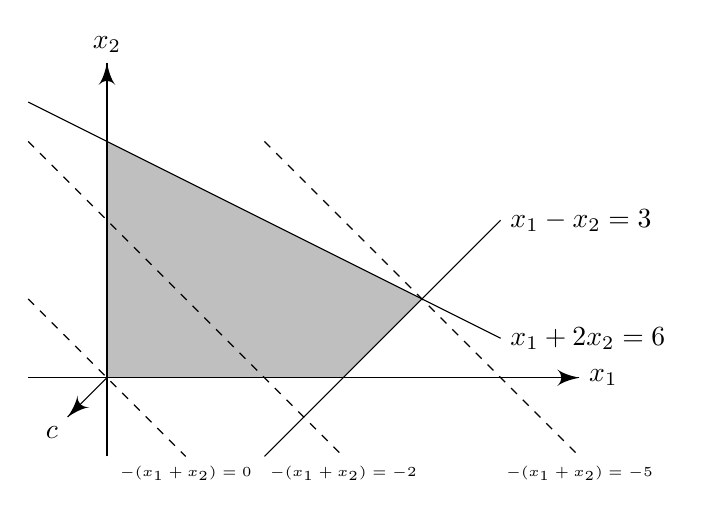
\begin{tikzpicture}
      \path [fill=gray!50!white] (0, 0) -- (3, 0) -- (4, 1) -- (0, 3) -- cycle;

      \draw [->] (-1, 0) -- (6, 0) node [right] {$x_1$};
      \draw [->] (0, -1) -- (0, 4) node [above] {$x_2$};

      \draw (2, -1) -- (5, 2) node [right] {$x_1 - x_2 = 3$};
      \draw (-1, 3.5) -- (5, 0.5) node [right] {$x_1 + 2x_2 = 6$};
      \draw [->] (0, 0) -- (-0.5, -0.5) node [anchor=north east] {$c$};

      \draw [dashed] (-1, 1) -- (1, -1) node [below] {\tiny $-(x_1 + x_2) = 0$};
      \draw [dashed] (-1, 3) -- (3, -1) node [below] {\tiny $-(x_1 + x_2) = -2$};
      \draw [dashed] (2, 3) -- (6, -1) node [below] {\tiny $-(x_1 + x_2) = -5$};
    \end{tikzpicture}
  \end{center}
  The shaded region is the feasible region, and $c$ is our \emph{cost vector}. The dotted lines, which are orthogonal to $c$ are lines in which the objective function is constant. To minimize our objective function, we want the line to be as right as possible, which is clearly achieved at the intersection of the two boundary lines.
\end{eg}
Now we have a problem. In the general case, we have absolutely \emph{no idea} how to solve it. What we \emph{do} know, is how to do \emph{un}constrained optimization.

\subsection{Review of unconstrained optimization}
Let $f: \R^n \to \R$, $x^*\in \R^n$. A necessary condition for $x^*$ to minimize $f$ over $\R^n$ is $\nabla f(x^*) = 0$, where
\[
  \nabla  f = \left(\frac{\partial f}{\partial x_1}, \cdots, \frac{\partial f}{\partial x_n}\right)^T
\]
is the gradient of $f$.

However, this is obviously not a sufficient condition. Any such point can be a maximum, minimum or a saddle. Here we need a notion of convexity:
\begin{defi}[Convex region]
  A region $S\subseteq \R^n$ is \emph{convex} iff for all $\delta\in [0, 1]$, $x, y\in S$, we have $\delta x + (1 - \delta) y \in S$. Alternatively, If you take two points, the line joining them lies completely within the region.

  \begin{center}
    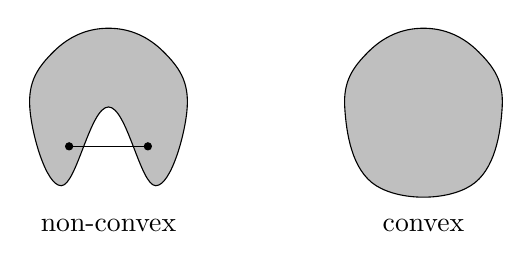
\begin{tikzpicture}
      \begin{scope}[shift={(-2, 0)}]
        \draw [fill=gray!50!white] plot [smooth cycle, tension=0.7] coordinates {(0, 1) (-0.7, 0.7) (-1, 0) (-0.6, -1) (0, 0) (0.6, -1) (1, 0) (0.7, 0.7)};
        \draw (-0.5, -0.5) node [circ] {} -- (0.5, -0.5) node [circ] {};

        \node at (0, -1.5) {non-convex};
      \end{scope}

      \begin{scope}[shift={(2, 0)}]
        \draw [fill=gray!50!white] plot [smooth cycle, tension=0.7] coordinates {(0, 1) (-0.7, 0.7) (-1, 0) (-0.6, -1) (0.6, -1) (1, 0) (0.7, 0.7)};
        \node at (0, -1.5) {convex};
      \end{scope}
    \end{tikzpicture}
  \end{center}
\end{defi}

\begin{defi}[Convex function]
  A function $f: S\to \R$ is \emph{convex} if for all $x, y\in S$, $\delta\in [0, 1]$, then $\delta f(x) + (1 - \delta)f(y) \geq f(\delta x + (1 - \delta)y)$.

  \begin{center}
    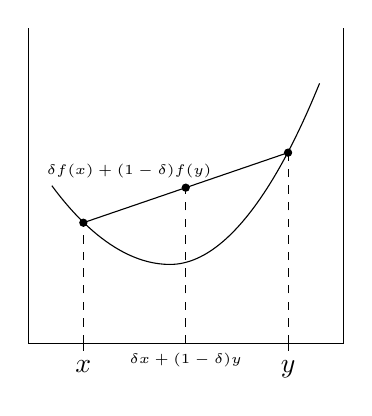
\begin{tikzpicture}
      \draw(-2, 4) -- (-2, 0) -- (2, 0) -- (2, 4);
      \draw (-1.3, 0.1) -- (-1.3, -0.1) node [below] {$x$};
      \draw (1.3, 0.1) -- (1.3, -0.1) node [below] {$y$};
      \draw (-1.7, 2) parabola bend (-.2, 1) (1.7, 3.3);
      \draw [dashed] (-1.3, 0) -- (-1.3, 1.53) node [circ] {};
      \draw [dashed] (1.3, 0) -- (1.3, 2.42) node [circ] {};
      \draw (-1.3, 1.53) -- (1.3, 2.42);
      \draw [dashed] (0, 0) node [below] {\tiny $\delta x + (1 - \delta)y$} -- (0, 1.975) node [above] {\tiny$\delta f(x) + (1 - \delta) f(y)\quad\quad\quad\quad\quad\quad$} node [circ] {};
    \end{tikzpicture}
  \end{center}

  A function is \emph{concave} if $-f$ is convex. Note that a function can be neither concave nor convex.
\end{defi}

We have the following lemma:
\begin{lemma}
  Let $f$ be twice differentiable. Then $f$ is convex on a convex set $S$ if the Hessian matrix
  \[
    Hf_{ij} = \frac{\partial^2 f}{\partial x_i \partial x_j}
  \]
  is positive semidefinite for all $x\in S$, where this fancy term means:
\end{lemma}

\begin{defi}[Positive-semidefinite]
  A matrix $H$ is \emph{positive semi-definite} if $v^T Hv \geq 0$ for all $v\in \R^n$.
\end{defi}

Which leads to the following theorem:
\begin{thm}
  Let $X\subseteq \R^n$ be convex, $f: \R^n \to \R$ be twice differentiable on $X$. If $x^* \in X$ satisfy $\nabla f(x^*) = 0$ and $Hf(x)$ is positive semidefinite for all $x\in X$, then $x^*$ minimizes $f$ on $X$.
\end{thm}
We will not prove these.

Note that this is helpful, since linear functions are convex (and concave). The problem is that our problems are constrained, not unconstrained. So we will have to convert constrained problems to unconstrained problems.

\section{The method of Lagrange multipliers}
The trick is to include the constraints into the objective function, so that things outside the constraint will not be thought to be minima.

Suppose the problem is
\begin{center}
  minimize $f(x)$ subject to $h(x) = b$, $x\in X$.
\end{center}
Call the constraint $(P)$.
\begin{defi}[Lagrangian]
  The \emph{Lagrangian} of a constraint $(P)$ is defined as
  \[
    L(x, \lambda) = f(x) - \lambda^T(h(x) - b).
  \]
  for $\lambda\in \R^m$.
\end{defi}
Note that when the constraint is satisfied, $h(x) - b = 0$, and $L(x, \lambda) = f(x)$.

We could as well have used
\[
  L(x, \lambda) = f(x) + \lambda^T(h(x) - b).
\]
since we just have to switch the sign of $\lambda$. So we don't have to worry about getting the sign of $\lambda$ wrong when defining the Lagrangian.

If we minimize $L$ over both $x$ and $\lambda$, then we will magically find the minimal solution subject to the constrains. Sometimes.

\begin{thm}[Lagrangian sufficiency]
  Let $x^*\in X$ and $\lambda^*\in \R^m$ such that
  \[
    L(x^* ,\lambda^*) = \inf_{x\in X}L(x, \lambda^*)\quad\text{and}\quad h(x^*) = b.
  \]
  Then $x^*$ is optimal for ($P$).

  Alternatively, if $x^*$ minimizes $L$ for a fixed $\lambda^*$, and $x^*$ satisfies the constraints, then $x^*$ minimizes $f$.
\end{thm}
This looks like a pretty powerful result, but it turns out that it is quite easy to prove.

\begin{proof}
  We first define the ``feasible set'': let $X(b) = \{x\in X: h(x) = b\}$, ie. the set of all $x$ that satisfies the constraints. Then
  \begin{align*}
    \min_{x\in X(b)} f(x) &= \min_{x\in X(b)} (f(x) - \lambda^{*T}(h(x) - b))\quad\text{ since $h(x) - b = 0$}\\
    &\geq \min_{x\in X} (f(x) - \lambda^{*T}(h(x) - b))\\
    &= f(x^*) - \lambda^{*T}(h(x^*) - b).\\
    &= f(x^*).
  \end{align*}
\end{proof}


\begin{eg}
  Minimize $x_1 + x_2 - 2x_3$ subject to
  \begin{align*}
    x_1 + x_2 + x_3 &= 5\\
    x_1^2 + x_2^2 = 4
  \end{align*}
  The Lagrangian is
  \begin{align*}
    L(x, \lambda) &= x_1 - x_2 - 2x_3 - \lambda_1(x_1 + x_2 + x_3 - 5) - \lambda_2 (x_1^2 + x_2^2 - 4)\\
    &= ((1 - \lambda_1)x_1 - 2\lambda_2 x_1^2) + ((-1 - \lambda_1)x_2 - \lambda_2 x_2^2) \\
    &+ (-2 - \lambda_1)x_3 + 5\lambda_1 + 4\lambda_2
  \end{align*}
  We want to pick a $\lambda^*$ and $x^*$ such that $L(x^*, \lambda^*)$ is minimal. Then for our $\lambda^*$, $L(x, \lambda^*)$  must have a finite minimum!

  We note that $(-2 - \lambda_1)x_3$ does not have a finite minimum unless $\lambda_1 = -2$, since $x_3$ can take any value. Also, the terms in $x_1$ and $x_2$ do not have a finite minimum unless $\lambda_2 < 0$.

  With these in mind, we find a minimum by setting all first derivatives to be $0$:
  \begin{align*}
    \frac{\partial L}{\partial x_1} &= 1 - \lambda_1 - 2\lambda_2 x_1 = 3 - 2\lambda_2x_1\\
    \frac{\partial L}{\partial x_2} &= -1 - \lambda_1 - 2\lambda_2 x_2 = 1 - 2\lambda_2 x_2
  \end{align*}
  Since these must be both $0$, we must have
  \[
    x_1 = \frac{3}{2\lambda_2}, \quad x_2 = \frac{1}{2\lambda_2}.
  \]
  To show that this is indeed a minimum, we look at the Hessian matrix:
  \[
    HL =
    \begin{pmatrix}
      -2\lambda_2 & 0\\
      0 & -2\lambda_2
    \end{pmatrix}
  \]
  which is positive semidefinite when $\lambda_2 < 0$, which is the condition we came up with at the beginning.

  Let $Y = \{\lambda: \R^2: \lambda_1 = -2, \lambda_2 < 0\}$ be our helpful values of $\lambda$.

  So we have shown above that for every $\lambda \in Y$, $L(x, \lambda)$ has a unique minimum at $x(\lambda) = (\frac{3}{2\lambda_2}, \frac{1}{2\lambda2}, x_3)^T$.

  Now all we have to do is find $\lambda$ and $x$ such that $x(\lambda)$ satisfies the functional constraints. The second constraint gives
  \[
    x_1^2 + x_2^2 = \frac{9}{4\lambda^2} + \frac{1}{4\lambda_2^2} = 4 \Leftrightarrow \lambda_2 = -\sqrt{\frac{5}{8}}.
  \]
  The first constraint gives
  \[
    x_3 = 5 - x_1 - x_2.
  \]
  So the theorem implies that
  \[
    x_1 = -3\sqrt{\frac{2}{5}},\quad x_2 = -\sqrt{\frac{2}{5}},\quad x_3 = 5 + 4\sqrt{\frac{2}{5}}.
  \]
\end{eg}
So far so good. But what if our functional constraint is an inequality? We will need slack variables.

To minimize $f(x)$ subject to $h(x) \leq b$, $x\in X$, we proceed as follows:
\begin{enumerate}
  \item Introduce slack variables to obtain the equivalent problem, to minimize $f(x)$ subject to $h(x) + z = b$, $x \in X$, $z \geq 0$.
  \item Compute the Lagrangian
    \[
      L(x, z, \lambda) = f(x) - \lambda^T(f(x) + z - b).
    \]
  \item Find
    \[
      Y = \left\{\lambda: \inf_{x\in X, z\geq 0}L(x, z, \lambda) > -\infty\right\}.
    \]
  \item For each $\lambda\in Y$, minimize $L(x, z, \lambda)$, ie. find
    \[
      x^*(\lambda)\in X,\quad z^*(\lambda) \geq 0
    \]
    such that
    \[
      L(x^*(\lambda), z^*(\lambda), \lambda) = \inf_{x\in X, z\geq 0} L(x, z, \lambda)
    \]
  \item Find $\lambda^*\in Y$ such that
    \[
      h(x^*(\lambda^*)) + z^*(\lambda^*) = b.
    \]
\end{enumerate}
Then by the Lagrangian sufficiency condition, $x^*(\lambda^*)$ is optimal for the constrained problem.

\subsection{Complementary Slackness}
If we introduce a slack variable $z$, we note that changing the value of $z_j$ does not affect our objective function, and we are allowed to pick any positive $z$. Hence if the corresponding Lagrange multiplier is $\lambda_j$, then we must have $(z^*(\lambda))_j \lambda_j = 0$. This is since by definition $z^*(\lambda)_j$ minimizes $z_j \lambda_j$. Hence if $z_j \lambda_j \not= 0$, we can tweak the values of $z_j$ to make a smaller $z_j \lambda_j$.

This makes our life easier since our search space is smaller.

\begin{eg}
  Consider the following problem:
  \begin{center}
    maximize $x_1 - 3x_2$ subject to
    \begin{align*}
      x_1^2 + x_2^2 + z_1 &= 4\\
      x_1 + x_2 + z_2 + z_2 &= 2\\
      z_1, z_2 &\geq 0.
    \end{align*}
  where $z_1, z_2$ are slack variables.
  \end{center}

  The Lagrangian is
  \[
    L(x, z, \lambda) = ((1 - \lambda_2)x_1 - \lambda_1 x_1^2) + ((-3 - \lambda_2)x_2 - \lambda_1 x_2^2) - \lambda_1 z_1 - \lambda_2 z_2 + 4\lambda_1 + 2\lambda_2.
  \]
  To ensure finite minimum, we need $\lambda_1, \lambda_2 \leq 0$.

  By complementary slackness, $\lambda_1 z_1 = \lambda_2 z_2 = 0$. We can then consider the cases $\lambda_1 = 0$ and $z_1 = 0$ separately, and save a lot of algebra.
\end{eg}

\subsection{Shadow prices}
We can understand Lagrange multipliers intuitively via the following theorem:
\begin{thm}[]
  Consider the problem
  \begin{center}
    minimize $f(x)$ subject to $h(x) = b$.
  \end{center}
  Here we assume all functions are continuously differentiable. Suppose that for each $b\in \R^n$, $\phi(b)$ is the optimal value of $f$ and $\lambda^*$ is the corresponding Lagrange multiplier. Then
  \[
    \frac{\partial \phi}{\partial b_i} = \lambda_i^*.
  \]
\end{thm}
Proof is omitted, as it is just a tedious application of chain rule etc.

This can be interpreted as follows: suppose we are a factory which is capable of producing $m$ different kinds of goods. Since we have finitely many resources, and producing stuff requires resources, $h(x) = b$ limits the amount of goods we can produce. Now of course, if we have more resources, ie. we change the value of $b$, we will be able to produce more/less stuff, and thus generate more profit. The change in profit per change in $b$ is given by $\frac{\partial \phi}{\partial b_i}$, which is the value of $\lambda$.

The result also holds when the functional constraints are inequality constraints. If the $i$th constraint holds with equality at the optimal solution, then the above reasoning holds. Otherwise, if it is not held with equality, then the Lagrange multiplier is $0$ by complementary slackness. Also, the partial derivative of $\phi$ with respect to $b_i$ also has to be $0$, since changing the upper bound doesn't affect us if we are not at the limit. So they are equal.
\subsection{Lagrange duality}
Consider the problem
\begin{center}
  minimize $f(x)$ subject to $h(x) = b$, $x\in X$.
\end{center}
Denote this as $P$.

The Lagrangian is
\[
  L(x, \lambda) = f(x) - \lambda^T (h(x) - b).
\]
Define the dual function $g: \R^m \to \R$ as
\[
  g(\lambda) = \inf_{x\in X}L(x, \lambda).
\]
ie, we fix $\lambda$, and see how small we can get $L$ to be. As before, let
\[
  Y = \{\lambda\in \R^n: g(\lambda) > -\infty\}.
\]
Then we have
\begin{thm}[Weak duality]
  If $x\in X(b)$ (ie. $x$ satisfies both the functional and regional constraints) and $\lambda \in Y$, then
  \[
    g(\lambda) \leq f(x).
  \]
  In particular,
  \[
    \sup_{\lambda\in Y}g(\lambda) \leq \inf_{x\in X(b)}f(x).
  \]
\end{thm}

\begin{proof}
  \begin{align*}
    g(\lambda) &= \inf_{x'\in X}L(x', \lambda)\\
    &\leq L(x, \lambda)\\
    &= f(x) - \lambda^T (h(x) - b)\\
    &= f(x).
  \end{align*}
\end{proof}

This suggests that we can solve a dual problem - instead of minimizing $f$, we can maximize $g$ subject to $\lambda\in Y$. Denote this problem as $(D)$. The original problem $(P)$ is called \emph{primal}.

\begin{defi}[Strong duality]
  $(P)$ and $(D)$ are said to satisfy \emph{strong duality} if
  \[
    \sup_{\lambda\in Y}g(\lambda) = \inf_{x\in X(b)}f(x).
  \]
\end{defi}
It turns out that problems satisfying strong duality are exactly those for which the method of Lagrange multipliers work.

\begin{eg}
  Again consider the problem to minimize $x_1 - x_2 - 2x_3$ subject to
  \begin{align*}
    x_1 + x_2 + x_3 &= 5\\
    x_1^2 + x_2^2 &= 4
  \end{align*}
  We saw that
  \[
    Y = \{\lambda\in \R^2: \lambda_1 = -2, \lambda_2 < 0\}
  \]
  and
  \[
    x^*(\lambda) = \left(\frac{3}{2\lambda_2}, \frac{1}{2\lambda_2}, 5 - \frac{4}{2\lambda_2}\right).
  \]
  The dual function is
  \[
    g(\lambda) = \inf_{x\in X} L(x, \lambda) = L(x^*(\lambda), \lambda) = \frac{10}{4\lambda_2} + 4\lambda_2 - 10.
  \]
  The dual is the problem to
  \begin{center}
    maximize $\frac{10}{4\lambda_2} + 4\lambda_2 - 10$ subject to $\lambda_2 < 0$.
  \end{center}
  The maximum is attained for
  \[
    \lambda_2 = -\sqrt{\frac{5}{8}}
  \]
  After calculating the values of $g$ and $f$, we can see that the primal and dual do have the same optimal value.
\end{eg}

Right now, what we've got isn't helpful, because we won't know if our problem satisfies strong duality!

\subsection{Supporting hyperplanes and convexity}
We use the fancy term ``hyperplane'' to denote planes in higher dimensions (in an $n$-dimensional space, a hyperplane has $n - 1$ dimensions).

\begin{defi}[Supporting hyperplane]
  A hyperplane $\alpha: \R^m \to \R$ is \emph{supporting} to $\phi$ at $b$ if $\alpha$ intersects $\phi$ at $b$ and  $\phi(c) \geq \alpha(c)$ for all $c$.

  \begin{center}
    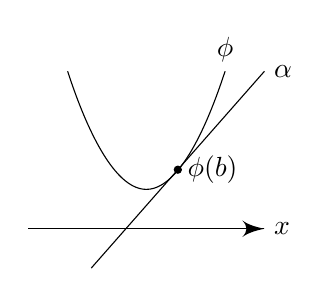
\begin{tikzpicture}
      \draw [->] (-1.5, 0) -- (1.5, 0) node [right] {$x$};
      \draw (-1, 2) parabola bend (0, 0.5) (1, 2) node [above] {$\phi$};
      \node [circ] at (0.4, 0.75) {};
      \node [right] at (0.4, 0.75) {$\phi(b)$};
      \draw (-0.7, -0.5) -- (1.5, 2) node [right] {$\alpha$};
    \end{tikzpicture}
  \end{center}
\end{defi}

\begin{thm}[]
  $(P)$ satisfies strong duality iff there exists a supporting hyperplane at $b$.
\end{thm}

\begin{proof}
  $(\Leftarrow)$ Suppose there is a supporting hyperplane. Then since the plane passes through $\phi(b)$, it must be of the form
  \[
    \alpha(c) = \phi(b) + \lambda^T(c - b).
  \]
  Since this is supporting, for all $c\in \R^m$,
  \[
    \phi(b) + \lambda^T(c - b) \leq \phi(c),
  \]
  or
  \[
    \phi(b) \leq \phi(c) - \lambda^T(c - b),
  \]
  This implies that
  \begin{align*}
    \phi(b) &\leq \inf_{c\in \R^m}(\phi(c) - \lambda^T(c - b))\\
    &= \inf_{c\in \R^m}\inf_{x\in X(c)}(f(x) - \lambda^T(h(x) - b))\\
    \intertext{(since $\phi(c) = \inf\limits_{x\in X(c)} f(x)$ and $h(x) = c$ for $x\in X(c)$)}
    &= \inf_{x\in X}L(x, \lambda).\\
    \intertext{(since $\bigcup\limits_{c\in \R^m}X(c) = X$, which is true since for any $x\in X$, we have $x\in X(h(x))$)}
    &= g(\lambda)
  \end{align*}
  By weak duality, $g(\lambda) \leq \phi(b)$. So $\phi(b) = g(\lambda)$. So strong duality holds.

  $(\Rightarrow)$. Assume now that we have strong duality. The there exists $\lambda$ such that for all $c\in \R^m$,
  \begin{align*}
    \phi(b) &= g(\lambda)\\
    &= \inf_{x\in X}L(x, \lambda)\\
    &\leq \inf_{x\in X(c)} L(x, \lambda)\\
    &= \inf_{x\in X(c)} (f(x) - \lambda^T(h(x) - b))\\
    &= \phi(c) - \lambda^T(c - b)
  \end{align*}
  So $\phi(b) + \lambda^T(c - b) \leq \phi(c)$. So this defines a supporting hyperplane.
\end{proof}

\begin{thm}[Supporting hyperplane theorem]
  Suppose that $\phi: \R^m \to \R$ is convex and $b\in\R^m$ lies in the interior of the set of points where $\phi$ is finite. Then there exists a supporting hyperplane to $\phi$ at $b$.
\end{thm}

We're having some progress, but this is still not helpful, since we don't know what $\phi$ is! So now we have a sufficient condition for Lagrange multipliers to work:
\subsection{A sufficient condition for convexity of \texorpdfstring{$\phi$}{phi}}
\begin{thm}
  Let
  \[
    \phi(b) = \inf_{x\in X} \{f(x): h(x) \leq b\}
  \]
  If $X, f, h$ are convex, then so is $\phi$ (assuming feasibility and boundedness).
\end{thm}

\begin{proof}
  Consider $b_1, b_2\in \R^m$ such that $\phi(b_1)$ and $\phi(b_2)$ are defined. Let $\delta \in [0, 1]$ and define $b = \delta b_1 + (1 - \delta)b_2$. We want to show that $\phi(b) \leq \delta \phi(b_1) + (1 - \delta)\phi(b_2)$.

  Consider $x_1 \in X(b_1)$, $x_2 \in X(b_2)$, and let $x = \delta x_1 + (1 - \delta)x_2$. By convexity of $X$, $x\in X$.

  By convexity of $h$,
  \begin{align*}
    h(x) &= h(\delta x_1 + (1 - \delta) x_2)\\
    &\leq \delta h(x_1) + (1 - \delta)h(x_2)\\
    &\leq \delta b_1 + (1 - \delta)b_2\\
    &= b
  \end{align*}
  So $x\in X(b)$. Since $\phi(x)$ is an optimal solution, by convexity of $f$,
  \begin{align*}
    \phi(b) &\leq f(x)\\
    &= f(\delta x_1 + (1 - \delta) x_2)\\
    &\leq \delta f(x_1) + (1 - \delta)f(x_2)
   \end{align*}
   This holds for any $x_1\in X(b_1)$ and $x_2 \in X(b_2)$. So by taking infimum of the right hand side,
   \[
     \phi(b) \leq \delta \phi(b_1) + (1 - \delta) \phi(b_2).
   \]
   So $\phi$ is convex.
\end{proof}
$h(x) = b$ is equivalent to $h(x) \leq b$ and $-h(x) \leq -b$. So the result holds for problems with equality constraints if both $h$ and $-h$ are convex, ie. if $h(x)$ is linear.

So
\begin{thm}[]
  If a linear program is feasible and bounded, then it satisfies strong duality.
\end{thm}

\section{Solutions of linear programs}
We first illustrate the general idea with the case of a 2D linear program

\begin{center}
  maximize $x_1 + x_2$ subject to
  \begin{align*}
    x_1 + 2x_2 &\leq 6\\
    x_1 - x_2 &\leq 3\\
    x_1, x_2 &\geq 0
  \end{align*}
\end{center}

We can plot the solution space out
\begin{center}
  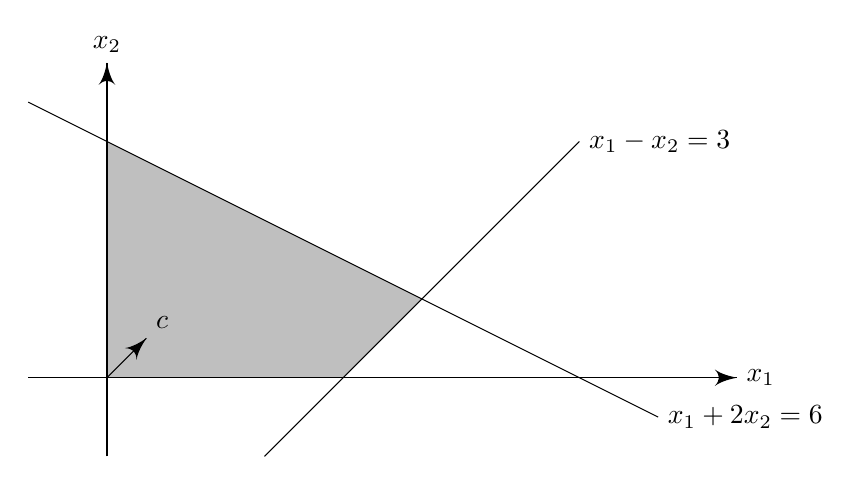
\begin{tikzpicture}
    \path [fill=gray!50!white] (0, 0) -- (3, 0) -- (4, 1) -- (0, 3) -- cycle;
    \draw [->] (-1, 0) -- (8, 0) node [right] {$x_1$};
    \draw [->] (0, -1) -- (0, 4) node [above] {$x_2$};

    \draw (2, -1) -- +(4, 4) node [right] {$x_1 - x_2 = 3$};
    \draw (-1, 3.5) -- +(8, -4) node [right] {$x_1 + 2x_2 = 6$};
    \draw [->] (0, 0) -- (0.5, 0.5) node [anchor=south west] {$c$};
  \end{tikzpicture}
\end{center}

To maximize $x_1 + x_2$, we want to go as far in the $c$ direction as possible. It should be clear that the optimal point will lie on a corner of the polygon of feasible region, no matter what the shape of it might be.

Even if we have cases where $c$ is orthogonal to one of the lines, eg
\begin{center}
  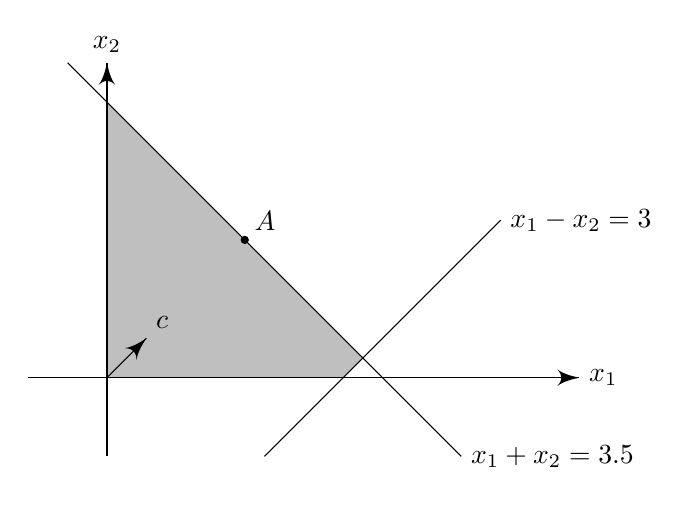
\begin{tikzpicture}
    \path [fill=gray!50!white] (0, 0) -- (3, 0) -- (3.25, 0.25) -- (0, 3.5) -- cycle;
    \draw [->] (-1, 0) -- (6, 0) node [right] {$x_1$};
    \draw [->] (0, -1) -- (0, 4) node [above] {$x_2$};

    \draw (2, -1) -- +(3, 3) node [right] {$x_1 - x_2 = 3$};
    \draw (-0.5, 4) -- +(5, -5) node [right] {$x_1 + x_2 = 3.5$};
    \draw [->] (0, 0) -- (0.5, 0.5) node [anchor=south west] {$c$};
    \node [circ] at (1.75, 1.75) {};
    \node at (1.75, 1.75) [anchor = south west] {$A$};
  \end{tikzpicture}
\end{center}
An optimal point might be $A$. However, if we know that $A$ is an optimal point, we can slide it across the $x_1 + x_2 = 3.5$ line until it meets one of the corners. Hence we know that one of the corners must be an optimal point.

\subsection{Basic solutions}
In general, if both the constraints and the objective functions are linear, then the optimal point always lies on a ``corner'', or an \emph{extreme point}.

\begin{defi}[Extreme point]
  An \emph{extreme point} $x\in S$ of a convex set $S$ is a point that cannot be written as a convex combination of two distinct points in $S$, ie. if $y, z\in S$ and $\delta \in (0, 1)$ satisfy
  \[
    x = \delta y + (1 - \delta) z,
  \]
  then $x = y = z$.
\end{defi}

Consider again the linear program in standard form, ie.
\begin{center}
  \emph{maximize} $c^T x$ subject to $Ax = b, x \geq 0$, where $A \in \R^{m\times n}$ and $b\in \R^m$.
\end{center}

\begin{defi}[Basic solution and basis]
  A solution $x\in \R^n$ is \emph{basic} if it has at most $m$ non-zero entries (out of $n$), ie. if there exists a set $B\subseteq \{1, \cdots, n\}$ with $|B| = m$ such that $x_i = 0$ if $i\not\in B$. In this case, $B$ is called the \emph{basis}, and $x_i$ are the \emph{basic variables} if $i\in B$.
\end{defi}

\begin{defi}[Non-degenerate solutions]
  A basic solution is \emph{non-degenerate} if it has exactly $m$ non-zero entries.
\end{defi}

\begin{defi}[Basic feasible solution]
  A basic solution $x$ is \emph{feasible} if it satisfies $x \geq 0$ (being a solution only requires $Ax = b$).
\end{defi}

\begin{eg}
  Consider the linear program
  \begin{center}
    maximize $f(x) = x_1 + x_2$ subject to
    \begin{align*}
      x_1 + 2x_2 + z_1&= 6\\
      x_1 - x_2 + z_2 &= 3\\
      x_1, x_2, z_1, z_2 &\geq 0
    \end{align*}
  \end{center}
  where we have included the slack variables.

  Since we have 2 constraints, a basic solution would require 2 non-zero entries, and thus 2 zero entries. The possible basic solutions are

  \begin{center}
    \begin{tabular}{cccccc}
      \toprule
      & $x_1$ & $x_2$ & $z_1$ & $z_2$ & $f(x)$\\
      \midrule
      $A$ & $0$ & $0$ & $6$ & $3$ & $0$\\
      $B$ & $0$ & $3$ & $0$ & $6$ & $3$\\
      $C$ & $4$ & $1$ & $0$ & $0$ & $5$\\
      $D$ & $3$ & $0$ & $3$ & $0$ & $3$\\
      $E$ & $6$ & $0$ & $0$ & $-4$ & $6$\\
      $F$ & $0$ & $-3$ & $12$ & $0$ & $-3$\\
      \bottomrule
    \end{tabular}
  \end{center}

  Among all 6, $E$ and $F$ are \emph{not} feasible solutions since they have negative entries. So the basic feasible solutions are $A, B, C, D$.

  \begin{center}
    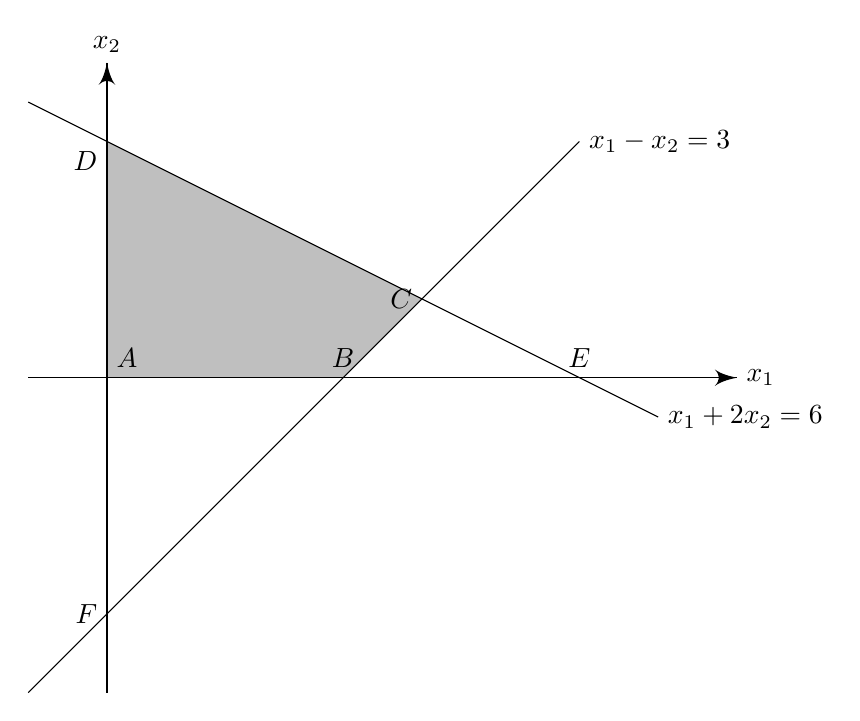
\begin{tikzpicture}
      \fill [fill=gray!50!white] (0, 0) node [anchor = south west] {$A$} --
      (3, 0) node [above] {$B$} --
      (4, 1) node [left] {$C$} --
      (0, 3) node [anchor = north east] {$D$} -- cycle;

      \draw [->] (-1, 0) -- (8, 0) node [right] {$x_1$};
      \draw [->] (0, -4) -- (0, 4) node [above] {$x_2$};

      \draw (-1, -4) -- +(7, 7) node [right] {$x_1 - x_2 = 3$};
      \draw (-1, 3.5) -- +(8, -4) node [right] {$x_1 + 2x_2 = 6$};
      \node [above] at (6, 0) {$E$};
      \node [left] at (0, -3) {$F$};
    \end{tikzpicture}
  \end{center}
\end{eg}

\subsection{Extreme points and optimal solutions}
Now we prove that the optimal solutions are exactly the basic feasible solutions.

Here we assume that the rows of $A$ are linearly independent, and any set of $m$ columns are linearly independent. Otherwise, just throw away the redundant rows or columns.

\begin{thm}[]
  A vector $x$ is a basic feasible solution of $Ax = b$ if and only if it is an extreme point of the set $X(b) = \{x': Ax' = b, x' \geq 0\}$.
\end{thm}
This is the generalization of the statement in 2D, and we are not going to prove this. What we will prove is the following:

\begin{thm}[]
  If $(P)$ is feasible and bounded, then there exists an optimal solution that is a basic feasible solution.
\end{thm}

\begin{proof}
  Let $x$ be optimal of $(P)$. If $x$ has at most non-zero entries, it is a basic feasible solution, and we are done.

  Now suppose $x$ has $r > m$ non-zero entries. Since it is not an extreme point, we have $y\not= z\in X(b)$, $\delta \in (0, 1)$ such that
  \[
    x = \delta y + (1 - \delta) z.
  \]
  We will show there exists an optimal solution strictly fewer than $r$ non-zero entries. Then the claim follows by induction.

  By optimality of $x$, we have $c^T x \geq c^T y$ and $c^T x \geq c^T z$.

  Since $c^T x = \delta c^T y + (1 - \delta)c^Tz$, we must have that $c^T x = c^T y = c^T z$, ie. $y$ and $z$ are also optimal.

  Since $y \geq 0$ and $z \geq 0$, $x = \delta y + (1 - \delta) z$ implies that $y_i = z_i = 0$ whenever $x_i = 0$.

  So the non-zero entries of $y$ and $z$ is a subset of the non-zero entries of $x$. So $y$ and $z$ have at most $r$ non-zero entries, which must occur in rows where $x$ is also non-zero.

  If $y$ or $z$ has strictly fewer than $r$ non-zero entries, then we are done. Otherwise, for any $\hat{\delta}$ (not necessarily in $(0, 1)$),let
  \[
    x_{\hat{\delta}} = \hat{\delta} y + (1 - \hat{\delta}) z = z + \hat{\delta}(y - z).
  \]
  Observe that $x_{\hat{\delta}}$ is optimal for every $\hat\delta\in \R$.

  Moreover, $y - z \not= 0$, and all non-zero entries of $y - z$ occur in rows where $x$ is non-zero as well. We can thus choose $\hat\delta\in \R$ such that $x_{\hat{\delta}} \geq 0$ and $x_{\hat{\delta}}$ has strictly fewer than $r$ non-zero entries.
\end{proof}
Intuitively, this is what we do when we ``slide along the line'' if $c$ is orthogonal to one of the boundary lines.

The latter result in fact holds more generally for the maximum of a convex function $f$ over a compact convex set $X$ (ie. closed and bounded).

In that case, we can write any point $x\in X$ as a convex combination
\[
  x = \sum_{i = 1}^k \delta_i x^i
\]
of extreme points $x^k\in X$, where $\delta \in \R_{\geq 0}^k$ and $\sum_{i=1}^k \delta_i = 1$.

Then, by convexity of $f$,
\[
  f(x) \leq \sum_{i = 1}^k \delta_i f(x^i) \leq \max_i f(x^i)
\]
So any point in the interior cannot be better than the extreme points.
\subsection{Linear programming duality}
Consider the linear program in general form with slack variables,

\begin{center}
  minimize $c^Tx$ subject to $Ax - z = b$, $x, z\geq 0$
\end{center}
We have $X = \{(x, z): x, z\geq 0\}\subseteq \R^{m + n}$.

The Lagrangian is
\[
  L(x, z, \lambda) = c^Tx - \lambda^T(A x - z - b) = (c^T - \lambda^TA)x + \lambda^T z + \lambda^T b.
\]
Since $x, z$ can be arbitrarily positive, this has a finite minimum if and only if
\[
  c^T - \lambda^TA \geq 0, \lambda^T \geq 0.
\]
Call the feasible set $Y$. Then for fixed $\lambda\in Y$, the minimum of $L(x, z, \lambda)$ is attained when $(c^T - \lambda^T A)x$ and $\lambda^T z = 0$ by complementary slackness. So
\[
  g(\lambda) = \inf_{(x, z) \in X} L(x, z, \lambda) = \lambda^T b.
\]
The dual is thus
\begin{center}
  maximize $\lambda^T b$ subject to $A^T\lambda \leq c, \lambda \geq 0$
\end{center}

\begin{thm}[]
  The dual of the dual of a linear program is the primal.
\end{thm}

\begin{proof}
  It suffices to show this for the linear program in general form. We have shown above that the dual problem is
  \begin{center}
    minimize $-b^T\lambda$ subject to $-A^T \lambda \geq -c, \lambda \geq 0$.
  \end{center}
  This problem has the same form as the primal, with $-b$ taking the role of $c$, $-c$ taking the role of $b$, $-A^T$ taking the role of $A$. So doing it again, we get back to the original problem.
\end{proof}

\begin{eg}
  Let the primal problem be
  \begin{center}
    maximize $3x_1 + 2x_2$ subject to
    \begin{align*}
      2x_1 + x_2 + z_1 &= 4\\
      2x_1 + 3x_2 + z_2 &= 6\\
      x_1, x_2, z_1, z_2 \geq 0.
    \end{align*}
  \end{center}
  Then the dual problem is
  \begin{center}
    minimize $4\lambda_1 + 6\lambda_2$ such that
    \begin{align*}
      2\lambda_1 + 2\lambda_2 - \mu_1 &= 3\\
      \lambda_1 + 3\lambda_2 - \mu_2 &= 2\\
      \lambda_1, \lambda_2, \mu_1, \mu_2 \geq 0.
    \end{align*}
  \end{center}
  We can compute all basic solutions of the primal and the dual by setting $n - m - 2$ variables to be zero in turn.

  Given a particular basic solutions of the primal, the corresponding solutions of the dual can be found by using the complementary slackness solutions:
  \[
    \lambda_1 z_1 = \lambda_2 z_2 = 0,\quad \mu_1 x_1 = \mu_2 x_2 = 0.
  \]
  \begin{center}
    \begin{tabular}{cccccccccccc}
      \toprule
      & $x_1$ & $x_2$ & $z_1$ & $z_2$ & $f(x)$ &\;& $\lambda_1$ & $\lambda_2$ & $\mu_1$ & $\mu_2$ & $g(\lambda)$\\
      \midrule
      A & 0 & 0 & 4 & 6 & 0 && 0 & 0 & -3 & -2 & 0\\
      B & 2 & 0 & 0 & 2 & 6 && $\frac{3}{2}$ & 0 & 0 & $-\frac{1}{2}$ & 6\\
      C & 3 & 0 & -2 & 0 & 9 && 0 & $\frac{3}{2}$  & 0 & $\frac{5}{2}$ & 9\\
      D & $\frac{3}{2}$ & 1 & 0 & 0 & $\frac{13}{2}$ && $\frac{5}{4}$ & $\frac{1}{4}$  & 0 & 0 & $\frac{13}{2}$\\
      E & 0 & 2 & 2 & 0 & 4 && 0 & $\frac{2}{3}$ & $-\frac{5}{3}$ & 0 & 4\\
      F & 0 & 4 & 0 & -6 & 8 && 2 & 0 & 1 & 0 & 8\\
      \bottomrule
    \end{tabular}
  \end{center}

  \begin{center}
    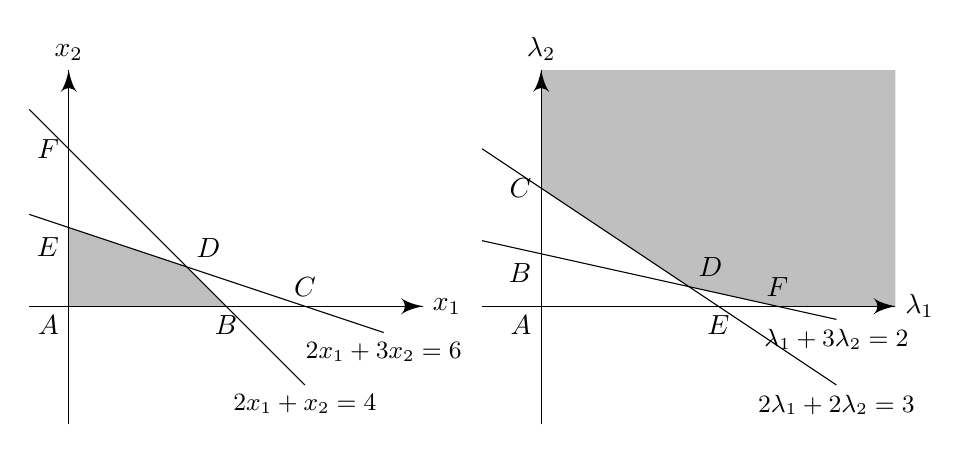
\begin{tikzpicture}
      \begin{scope}[yscale=0.5]
        \path [fill=gray!50!white] (0, 0) node [anchor = north east] {$A$} --
        (2, 0) node [below] {$B$} --
        (1.5, 1) node [anchor = south west] {$D$} --
        (0, 2) node [anchor = north east] {$E$} -- cycle;
        \node [above] at (3, 0) {$C$};
        \node [left] at (0, 4) {$F$};

        \draw [->] (-0.5, 0) -- (4.5, 0) node [right] {$x_1$};
        \draw [->] (0, -3) -- (0, 6) node [above] {$x_2$};
        \draw (-0.5, 5) -- +(3.5, -7) node [below] {\small $2x_1 + x_2 = 4$};
        \draw (-0.5, 2.333) -- +(4.5, -3) node [below] {\small $2x_1 + 3x_2 = 6$};
      \end{scope}

      \begin{scope}[shift={(6, 0)}, xscale=1.5]
        \path [fill=gray!50!white] (0, 3) -- (0, 1.5) node [left] {$C$} --
        (1.25, 0.25) node [anchor = south west] {$D$} --
        (2, 0) node [above] {$F$} --
        (3, 0) -- (3, 3) -- cycle;
        \node at (0, 0) [anchor = north east] {$A$};
        \node at (0, 0.667) [anchor = north east] {$B$};
        \node at (1.5, 0) [below] {$E$};

        \draw [->] (-0.5, 0) -- (3, 0) node [right] {$\lambda_1$};
        \draw [->] (0, -1.5) -- (0, 3) node [above] {$\lambda_2$};

        \draw (-0.5, 2) -- +(3, -3) node [below] {\small $2\lambda_1 + 2\lambda_2 = 3$};
        \draw (-0.5, 0.833) -- +(3, -1) node [below] {\small $\lambda_1 + 3\lambda_2 = 2$};
      \end{scope}

    \end{tikzpicture}
  \end{center}

  We see that $D$ is the only solution such that both the primal and dual solutions are feasible. So we know it is optimal without even having to calculate $f(x)$. It turns out this is always the case.
\end{eg}

\begin{thm}[]
  Let $x$ and $\lambda$ be feasible for the primal and the dual of the linear program in general form. Then $x$ and $\lambda$ and optimal if and only if they satisfy complementary slackness, ie. if
  \[
    (c^T - \lambda^T A)x = 0\text{ and }\lambda^T(Ax - b) = 0.
  \]
\end{thm}

\begin{proof}
  If $x$ and $\lambda$ are optimal, then
  \[
    c^Tx = \lambda^T b
  \]
  since every linear program satisfies strong duality. So
  \begin{align*}
    c^Tx &= \lambda^T b\\
    &= \inf_{x'\in X} (c^T x' - \lambda^T(Ax' - b))\\
    &\leq c^T - \lambda^T (Ax - b)\\
    &\leq c^T x
  \end{align*}
  since $Ax \geq b$ and $\lambda\geq 0$.

  The first and last term are the same. So the inequalities hold with equality. Therefore
  \[
    \lambda^T b = c^Tx - \lambda^T (Ax - b) = (c^T - \lambda^TA)x + \lambda^Tb.
  \]
  So
  \[
    (c^T - \lambda^TA)x = 0.
  \]
  Also,
  \[
    c^Tx - \lambda^T(Ax - b) = c^Tx
  \]
  implies
  \[
    \lambda^T(Ax - b) = 0.
  \]
  On the other hand, suppose we have complementary slackness, ie.
  \[
    (c^T - \lambda^T A)x = 0\text{ and }\lambda^T(Ax - b) = 0,
  \]
  then
  \[
    c^Tx = c^Tx - \lambda^T(Ax - b) = (c^T - \lambda^T A)x + \lambda^T b = \lambda^Tb.
  \]
  Hence by weak duality, $x$ and $\lambda$ are optimal.
\end{proof}
\subsection{Simplex method}
We start with an example, showing what we do, then explain the logic behind, then do a more proper example.

\begin{eg}
  Consider the following problem:
  \begin{center}
    Maximize $x_1 + x_2$ subject to
    \begin{align*}
      x_1 + 2x_2 + z_1 &= 6\\
      x_1 - x_2 + z_2 &= 3\\
      x_1, x_2, z_1, z_2 \geq 0.
    \end{align*}
  \end{center}

  We write everything in the \emph{simplex tableau}, by noting down the coefficients:
  \begin{center}
    \begin{tabular}{cccccc}
      \toprule
      &$x_1$ & $x_2$ & $z_1$ & $z_2$ \\
      \midrule
      Constraint 1 & 1 & 2 & 1 & 0 & 6 \\
      Constraint 2 & 1 & -1 & 0 & 1 & 3 \\
      Objective & 1 & 1 & 0 & 0 & 0 \\
      \bottomrule
    \end{tabular}
  \end{center}
  We see an identity matrix $\begin{pmatrix} 1 & 0\\ 0 & 1\end{pmatrix}$ in the $z_1$ and $z_2$ columns, and these correspond to basic feasible solution: $z_1 = 6, z_2 = 3, x_1 = x_2 = 0$. It's pretty clear that our basic feasible solution is not optimal, since our objective function is $0$. This is since something in the last row is positive, and we can increase the objective by, say, increasing $x_1$.

  The simplex method says that we can find the optimal solution if we make the bottom row all negative while keeping the right column positive, by doing row operations.

  We multiply the first row by $\frac{1}{2}$ and subtract/add it to the other rows to obtain
  \begin{center}
    \begin{tabular}{cccccc}
      \toprule
      &$x_1$ & $x_2$ & $z_1$ & $z_2$ & \\
      \midrule
      Constraint 1 & $\frac{1}{2}$ & 1 & $\frac{1}{2}$ & 0 & 3 \\
      Constraint 2 & $\frac{2}{3}$ & 0 & $\frac{1}{2}$ & 1 & 6 \\
      Objective & $\frac{1}{2}$ & 0 & $-\frac{1}{2}$ & 0 & -3\\
      \bottomrule
    \end{tabular}
  \end{center}
  Our new basic feasible solution is $x_2 = 3, z_2 = 6, x_1 = z_1 = 0$. We see that the number in the bottom-right corner is $-f(x)$. We can continue this process to finally obtain a solution.
\end{eg}
Here we adopt the following notation: let $A\subseteq \R^{m\times n}$ and $b\in \R^m$. Assume that $A$ has full rank. Let $B$ be a basis and set $B\subseteq \{1, 2, \cdots, n\}$ with $|B| = m$, corresponding to at most $m$ non-zero entries.

We rearrange the columns so that all basis columns are on the left. Then we can write our matrices as
\begin{align*}
  A_{m\times n} &=
  \begin{pmatrix}
    (A_B)_{m\times m} & (A_N)_{m\times (n - m)}
  \end{pmatrix}\\
  x_{n\times 1} &=
  \begin{pmatrix}
    (x_B)_{m\times 1} & (x_N)_{(n - m)\times 1}
  \end{pmatrix}^T\\
  c_{1\times n} &=
  \begin{pmatrix}
    (c_B)_{m\times 1} & (c_N)_{(n - m)\times 1}
  \end{pmatrix}.
\end{align*}

Then the functional constraints
\[
  Ax = b
\]
can be decomposed as
\[
  A_Bx_B + A_Nx_N = b.
\]
We can rearrange this to obtain
\[
  x_B = A_B^{-1}(b - A_N x_N).
\]
In particular, when $x_N = 0$, then
\[
  x_B = A_B^{-1}b.
\]
The general tableau is then
\begin{center}
  \begin{tabular}{ccc}
    \toprule
    Basis components & Other components\\
    \midrule\\
    $A_B^{-1} A_B = I$ & $A_B^{-1}A_N$ & $A_B^{-1}b$\\\\
    \midrule
    \quad$c^T_B - c^T_BA_B^{-1}A_B = 0$\quad & \quad$c_N^T - c_B^TA_B^{-1}A_N$\quad & $-c_B^T A_B^{-1}b$\\
    \bottomrule
  \end{tabular}
\end{center}
This might look really scary, and it is! Without caring too much about how the formulas for the cells come from, we see the identity matrix on the left, which is where we find our basic feasible solution. Below that is the row for the objective function. The values of this row must be $0$ for the basis columns.

On the right-most column, we have $A_B^{-1}b$, which is our $x_B$. Below that is $-c_B^TA_B^{-1}b$, which is the negative of our objective function $c_B^Tx_B$.
\subsubsection{The simplex tableau}
We have
\begin{align*}
  f(x) &= c^T x \\
  &= c_B^T x_B + c_N^T x_N\\
  &= c_B^T A_B^{-1}(b - A_N x_N) + c_N^T x_N\\
  &= c_B^T A_B^{-1}b + (c_N^T - c_B^TA_B^{-1}A_N)x_N.
\end{align*}
We will maximize $c^T x$ by choosing a basis such that $c_N^T - c_B^T A_B^{-1}A_N \leq 0$, ie. non-positive everywhere and $A_B^{-1}b \geq 0$.

If this is true, then for any feasible solution $x\in \R^n$, we must have $x_N \geq 0$. So $(c_N^T - c_B^TA_B^{-1}A_N)x_N \leq 0$ and
\[
  f(x) \leq c_B^T A_B^{-1}b.
\]
So if we choose $x_B = A_B^{-1}b$, $x_N = 0$, then we have an optimal solution.

Hence our objective is to pick a basis that makes $c_N^T - c_B^T A_B^{-1}A_N \leq 0$ while keeping $A_B^{-1}b \geq 0$. To do this, suppose this is not attained. Say $(c_N^T - c_B^T A_B^{-1}A_N)_i > 0$.

We can increase the value of the objective function by increasing $(x_N)_i$. As we increase $(x_N)_i$, we have to satisfy the functional constraints. So the value of other variables will change as well. We can keep increasing $(x_N)_i$ until another variable hits $0$, say $(x_B)_j$. Then we will have to stop.

However, if it so happens that we can increase $(x_N)_i$ indefinitely without other things hitting $0$, our problem is unbounded.

The effect of this is that we have switched basis by removing $(x_B)_j$ and adding $(x_N)_i$. We can continue from here. If $(c_N^T - c_B^T A_B^{-1}A_N)$ is negative, we are done. Otherwise, we continue the above procedure.

The simplex method is a systematic way of doing the above procedure.

\subsubsection{Using the Tableau}
Consider a tableau of the form
\begin{center}
\begin{tabular}{cc}
  \toprule\\
  \quad\quad $a_{ij}$\quad\quad\quad & $a_{i0}$\\\\
  \midrule
  \quad\quad $a_{0j}$\quad\quad\quad & $a_{00}$\\
  \bottomrule
\end{tabular}
\end{center}
where $a_{i0}$ is $b$, $a_{0j}$ corresponds to the objective function, and $a_{00}$ is initial $0$.

The simplex method proceeds as follows:
\begin{enumerate}
  \item Find an initial basic feasible solution.
  \item Check whether $a_{0j} \leq 0$ for every $j$. If so, the current solution is optimal. Stop.
  \item If not, choose a \emph{pivot column} $j$ such that $a_{0j} > 0$. Choose a \emph{pivot row} $i\in \{i: a_{ij} > 0\}$ that minimizes $a_{i0}/a_{ij}$. If multiple rows are minimize $a_{i0}/a_{ij}$, then the problem is degenerate, and things \emph{might} go wrong. If $a_{ij} \leq 0$ for all $i$, ie. we cannot choose a pivot row, the problem is unbounded, and we stop.
  \item We update the tableau by multiplying row $i$ by $1/a_{ij}$ (such that the new $a_{ij} = 1$), and add a $(-a_{kj}/a_{ij})$ multiple of row $i$ to each row $k \not= i$, including $k = 0$ (so that $a_{kj} = 0$ for all $k \not= i$)

    We have a basic feasible solution, since our choice of $a_{ij}$ makes all right-hand columns positive after subtracting (apart from $a_{00}$).
  \item \texttt{GOTO} (ii).
\end{enumerate}

Now visit the example at the beginning of the section to see how this is done in practice. Then read the next section for a more complicated example.
\subsection{The two-phase simplex method}
Sometimes we don't have a nice identity matrix to start with. In this case, we need to use the \emph{two-phase simplex method} to first find our first basic feasible solution, then to the actual optimization.

This method is illustrated by example.
\begin{eg}
  Consider the problem
  \begin{center}
    minimize $6x_1 + 3x_2$ subject to
    \begin{align*}
      x_1 + x_2 &\geq 1\\
      2x_1 - x_2 &\geq 1\\
      3x_2 &\leq 2\\
      x_1, x_2 &\geq 0
    \end{align*}
  \end{center}
  This is a minimization problem. To avoid being confused, we maximize $-6x_1 - 3x_2$ instead. We add slack variables to obtain
  \begin{center}
    maximize $-6x_1 - 3x_2$ subject to
    \begin{align*}
      x_1 + x_2  - z_1 &= 1\\
      2x_1 - x_2 - z_2 &= 1\\
      3x_2  + z_3 &= 2\\
      x_1, x_2, z_1, z_2, z_3 &\geq 0
    \end{align*}
  \end{center}
  Now we don't have a basic feasible solution, since we would need $z_1 = z_2 = -1, z_3 = 2$, which is not feasible. So we add \emph{more} variables, called the artificial variables.
  \begin{center}
    maximize $-6x_1 - 3x_2$ subject to
    \begin{align*}
      x_1 + x_2  - z_1 + y_1&= 1\\
      2x_1 - x_2 - z_2 +y_2 &= 1\\
      3x_2  + z_3 &= 2\\
      x_1, x_2, z_1, z_2, z_3, y_1, y_2 &\geq 0
    \end{align*}
  \end{center}
  Note that adding $y_1$ and $y_2$ might create new solutions, which is bad. We solve this problem by first trying to make $y_1$ and $y_2$ both $0$ and find a basic feasible solution. Then we can throw away $y_1$ and $y_2$ and then get a basic feasible for our original problem. So momentarily, we want to solve
  \begin{center}
   minimize $y_1 + y_2$ subject to
    \begin{align*}
      x_1 + x_2  - z_1 + y_1&= 1\\
      2x_1 - x_2 - z_2 +y_2&= 1\\
      3x_2  + z_3 &= 2\\
      x_1, x_2, z_1, z_2, z_3, y_1, y_2 &\geq 0
    \end{align*}
  \end{center}
  By minimizing $y_1$ and $y_2$, we will make them zero.

  Our simplex tableau is
  \begin{center}
    \begin{tabular}{cccccccc}
      \toprule
      $x_1$ & $x_2$ & $z_1$ & $z_2$ & $z_3$ & $y_1$ & $y_2$ \\
      \midrule
      1 & 1 & -1 & 0 & 0 & 1 & 0 & 1\\
      2 & -1 & 0 & -1 & 0 & 0 & 1 & 1\\
      0 & 3 & 0 & 0 & 1 & 0 & 0 & 2\\
      \midrule
      -6 & -3 & 0 & 0 & 0 & 0 & 0 & 0\\
      0 & 0 & 0 & 0 & 0 & -1 & -1 & 0\\
      \bottomrule
    \end{tabular}
  \end{center}
  Note that we keep both our original and ``kill-$y_i$'' objectives, but now we only care about the second one. We will keep track of the original objective so that we can use it in the second phase.

  We see an initial feasible solution $y_1 = y_2 = 1, z_3 = 2$. However, this is not a proper simplex tableau, as the basis columns should not have non-zero entries (apart from the identity matrix itself). But we have the two $-1$s at the bottom! So we add the first two rows to the last to obtain
  \begin{center}
    \begin{tabular}{cccccccc}
      \toprule
      $x_1$ & $x_2$ & $z_1$ & $z_2$ & $z_3$ & $y_1$ & $y_2$ \\
      \midrule
      1 & 1 & -1 & 0 & 0 & 1 & 0 & 1\\
      2 & -1 & 0 & -1 & 0 & 0 & 1 & 1\\
      0 & 3 & 0 & 0 & 1 & 0 & 0 & 2\\
      \midrule
      -6 & -3 & 0 & 0 & 0 & 0 & 0 & 0\\
      3 & 0 & -1 & -1 & 0 & 0 & 0 & 2\\
      \bottomrule
    \end{tabular}
  \end{center}
  Our pivot column is $x_1$, and our pivot row is the second row. We divide it by $1 $ and add/subtract it from other rows.

  \begin{center}
    \begin{tabular}{cccccccc}
      \toprule
      $x_1$ & $x_2$ & $z_1$ & $z_2$ & $z_3$ & $y_1$ & $y_2$ \\
      \midrule
      0 & $\frac{3}{2}$ & -1 & $\frac{1}{2}$ & 0 & 1 & $-\frac{1}{2}$ & $\frac{1}{2}$\\
      1 & $-\frac{1}{2}$ & 0 & $-\frac{1}{2}$ & 0 & 0 & $\frac{1}{2}$ & $\frac{1}{2}$\\
      0 & 3 & 0 & 0 & 1 & 0 & 0 & 2\\
      \midrule
      0 & -6 & 0 & -3 & 0 & 0 & 3 & 3\\
      0 & $\frac{3}{2}$ & $-1$ & $\frac{1}{2}$ & 0 & 0 & $-\frac{3}{2}$ & $\frac{1}{2}$\\
      \bottomrule
    \end{tabular}
  \end{center}
  There are two possible pivot columns. We pick $z_2$ and the first row as the pivot row.
  \begin{center}
    \begin{tabular}{cccccccc}
      \toprule
      $x_1$ & $x_2$ & $z_1$ & $z_2$ & $z_3$ & $y_1$ & $y_2$ \\
      \midrule
      0 & 3 & -2 & 1 & 0 & 2 & -1 & 1\\
      1 & 1 & -1 & 0 & 0 & 1 & 0 & 1\\
      0 & 3 & 0 & 0 & 1 & 0 & 0 & 2\\
      \midrule
      0 & 3 & -6 & 0 & 0 & 6 & 0 & 6\\
      0 & 0 & 0 & 0 & 0 & -1 & -1 & 0\\
      \bottomrule
    \end{tabular}
  \end{center}
  We see that $y_1$ and $y_2$ are no longer in the basis, and hence take value $0$. So we drop all the phase I stuff, and are left with
  \begin{center}
    \begin{tabular}{cccccccc}
      \toprule
      $x_1$ & $x_2$ & $z_1$ & $z_2$ & $z_3$\\
      \midrule
      0 & 3 & -2 & 1 & 0 & 1\\
      1 & 1 & -1 & 0 & 0 & 1\\
      0 & 3 & 0 & 0 & 1 & 2\\
      \midrule
      0 & 3 & -6 & 0 & 0 & 6\\
      \bottomrule
    \end{tabular}
  \end{center}
  We see a basic feasible solution $z_1 = x_1 = 1, z_3 = 2$.

  We pick $x_2$ as the pivot column, and the first row as the pivot row. Then we have
  \begin{center}
    \begin{tabular}{cccccccc}
      \toprule
      $x_1$ & $x_2$ & $z_1$ & $z_2$ & $z_3$\\
      \midrule
      0 & 1 & $-\frac{2}{3}$ & $\frac{1}{3}$ & 0 & $\frac{1}{3}$\\
      1 & 0 & $-\frac{1}{3}$ & $-\frac{1}{3}$ & 0 & $\frac{2}{3}$\\
      0 & 0 & 2 & -1 & 1 & 1\\
      \midrule
      0 & 0 & -4 & -1 & 0 & 5\\
      \bottomrule
    \end{tabular}
  \end{center}
  Since the last row is all negative, we have complementary slackness. So this is a optimal solution. So $x_1 = \frac{2}{3}, x_2 = \frac{1}{3}, z_3 = 1$ is a feasible solution, and our optimal value is $5$.

  Note that we previously said that the bottom right entry is the negative of the optimal value, not the optimal value itself! This is correct, since in the tableau, we are maximizing $-6x_1 - 3x_2$, whose maximum value is $-5$. So the minimum value of $6x_1 + 3x_2$ is $5$.
\end{eg}
\section{Non-cooperative games}
Here we have a short digression to game theory. We mostly focus on games with two players.

\subsection{Games and Solutions}
\begin{defi}[Bimatrix game]
  A two-player game, or \emph{bimatrix game}, is given by two matrices $P, Q\in \R^{m\times n}$. Player 1, or the \emph{row player}, chooses a row $i\in \{1, \cdots, m\}$, while player 2, the \emph{column player}, chooses a column $j\in \{1, \cdots, n\}$. These are selected without knowledge of the other player's decisions. The two players then get payoffs $P_{ij}$ and $Q_{ij}$ respectively.
\end{defi}

\begin{defi}[Strategy]
  Players are allowed to play randomly. The set of \emph{strategies} the row player can have is
  \[
    X = \{x\in \R^m: x \geq 0, \sum x_i = 1\}
  \]
  and the column player has strategies
  \[
    Y = \{y\in \R^n: y \geq 0, \sum y_i = 1\}
  \]
  Each vector corresponds to the probabilities of selecting each row or column.

  A strategy profile $(x, y)\in X\times Y$ induces a lottery, and we write $p(x, y) = x^T Py$ for the expected payoff of the row player.

  If $x_i = 1$ for some $i$, ie. we always pick $i$, we call $x$ a \emph{pure strategy}.
\end{defi}

\begin{eg}[Prisoner's dilemma]
  Suppose Alice and Bob commit a crime together, and are caught by the police. They can choose to remain silent ($S$) or testify ($T$). Different options will lead to different outcomes:
  \begin{itemize}
    \item Both keep silent: the police has little evidence and they go to jail for 2 years.
    \item One testifies and one remains silent: the one who testifies gets awarded and is freed, while the other gets stuck in jail for 10 years.
    \item Both testify: they both go to jail for 5 years.
  \end{itemize}

  We can represent this by a payoff table:
  \begin{center}
    \begin{tabular}{ccc}
      \toprule
      & $S$ & $T$\\
      \midrule
      $S$ & $(2, 2)$ & $(0, 3)$\\
      $T$ & $(3, 0)$ & $(1, 1)$\\
      \bottomrule
    \end{tabular}
  \end{center}
  For example, if the row player chooses $S$ and the column player chooses $T$, then the payoff of the row player is $0$ and the payoff of the column player is $3$.

  Note that higher payoff is desired, so a longer serving time corresponds to a lower payoff. Also, payoffs are interpreted relatively, so replacing $(0, 3)$ with $(0, 100)$ (and $(3, 0)$ with $(100, 0)$) in the payoff table would make no difference.

  Here we see that regardless of what the other person does, it is always strictly better to testify than not (unless you want to be nice). We say $T$ is a \emph{dominant strategy}, and $(1, 1)$ is \emph{Pareto dominated} by $(2, 2)$.
\end{eg}

\begin{eg}[Chicken]
  The game of \emph{Chicken} is as follows: two people drive their cars towards each other at high speed. If they collide, they will die. Hence they can decide to chicken out ($C$) or continue driving ($D$). If both don't chicken, they die, which is bad. If one chickens and the other doesn't the person who chicken looks silly (but doesn't die). If both chicken out, they both look slightly silly. This can be represented by the following table:
  \begin{center}
    \begin{tabular}{ccc}
      \toprule
      & $C$ & $D$ \\
      \midrule
      $C$ & $(2, 2)$ & $(1, 3)$ \\
      $D$ & $(3, 1)$ & $(0, 0)$\\
      \bottomrule
    \end{tabular}
  \end{center}
  Here there is no dominating strategy, so we need a different way of deciding what to do.

  Instead, we define the \emph{security level} of the row player to be
  \[
    \max_{x\in X}\min_{y\in Y} p(x, y) = \max_{x\in X}\min_{j\in \{1, \ldots, n\}} \sum_{i = 1}^m x_i p_{ij}.
  \]
  This is the strategy the row player can employ that minimizes the possible loss. This is called the maximin strategy.

  We can formulate this as a linear program:
  \begin{center}
    maximize $v$ such that
    \begin{align*}
      \sum_{i = 1}^m x_i p_{ij} &\geq v\quad\text{for all }j = 1, \cdots, n\\
      \sum_{i = 1}^m x_i &= 1\\
      x &\geq 0
    \end{align*}
  \end{center}
  Here the maximin strategy is to chicken. However, this isn't really what we are looking for, since if both players employ this maximin strategy, it would be better for you to not chicken out.
\end{eg}

\begin{defi}[Best response and equilibrium]
  A strategy $x\in X$ is a \emph{best response} to $y\in Y$ if for all $x'\in X$
  \[
    p(x, y) \geq p(x', y)
  \]
  A pair $(x, y)$ is an \emph{equilibrium} if $x$ is the best response against $y$ and $y$ is a best response against $x$.
\end{defi}

\begin{eg}
  In the chicken game, there are two pure equilibrium, $(3, 1)$ and $(1, 3)$, and there is a mixed equilibrium in which the players pick the options with equal probability.
\end{eg}

\begin{thm}[Nash, 1961]
  Every bimatrix game has an equilibrium.
\end{thm}

\subsection{The minimax theorem}
\begin{defi}[Zero-sum game]
  A bimatrix game is a \emph{zero-sum game}, or matrix game, if $q_{ij} = -p_{ij}$ for all $i, j$, ie. the total payoff is always 0.
\end{defi}
To specify a matrix game, we only need one matrix, not two, since the matrix of the other player is simply the negative of the matrix of the first.

\begin{thm}[von Neumann, 1928]
  If $P\in \R^{m\times n}$. Then
  \[
    \max_{x\in X}\min_{y\in Y} p(x, y) = \min_{y\in Y}\max_{x\in X} p(x, y).
  \]
  Note that this is equivalent to
  \[
    \max_{x\in X}\min_{y\in Y} p(x, y) = -\max_{y\in Y}\min_{x\in X} -p(x, y).
  \]
  The left hand side is the worst payoff the row player can get if he employs the minimax strategy. The right hand side is the worst payoff the column player can get if he uses his minimax strategy.

  The theorem says that if both players employ the minimax strategy, then this is an equilibrium.
\end{thm}

\begin{proof}
  Recall that the optimal value of $\max\min p(x, y)$ is a solution to the linear program
  \begin{center}
    maximize $v$ such that
    \begin{align*}
      \sum_{i = 1}^m x_i p_{ij} &\geq v\quad\text{for all }j = 1, \cdots, n\\
      \sum_{i = 1}^m x_i &= 1\\
      x &\geq 0
    \end{align*}
  \end{center}
  Adding slack variable $z\in \R^n$ with $z \geq 0$, we obtain the Lagrangian
  \[
    L(v, x, z, w, y) = v + \sum_{j = 1}^n y_j\left(\sum_{i = 1}^m x_ip_{ij} - z_j - v\right) - w\left(\sum_{i = 1}^m x_i - 1\right),
  \]
  where $w\in \R$ and $y\in \R^n$ are Lagrange multipliers. This is equal to
  \[
    \left(1 - \sum_{j = 1}^n y_j\right)v + \sum_{i = 1}^m \left(\sum_{j = 1}^n p_{ij}y_j - w\right)x_i- \sum_{j = 1}^n y_j z_j + w.
  \]
  This has finite minimum for all $v\in \R, x \geq 0$ iff $\sum y_i = 1$, $\sum p_{ij}y_j \leq w$ for all $i$, and $y \geq 0$. The dual is therefore
  \begin{center}
    minimize $w$ subject to
    \begin{align*}
      \sum_{j = 1}^n p_{ij}y_j &\leq w\quad\text{ for all }i\\
      \sum_{j = 1}^n {y_j} &= 1\\
      y &\geq 0
    \end{align*}
  \end{center}
  This corresponds to the column player choosing a strategy $(y_i)$ such that the expected payoff is bounded above by $w$.

  The optimum value of the dual is $\displaystyle\min_{y\in Y}\max_{x\in X}p(x, y)$. So the result follows from strong duality.
\end{proof}

In general, the equilibrium are given by
\begin{thm}
  $(x, y)\in X\times Y$ is an equilibrium of the matrix game with payoff matrix $P$ if and only if
  \begin{align*}
    \min_{y'\in Y} p(x, y') &= \max_{x' \in X}\min_{y'\in Y} p(x', y')\\
    \max_{x'\in X} p(x', y) &= \min_{y' \in Y}\max_{x'\in X} p(x', u')
  \end{align*}
  ie. the $x, y$ are optimizers for the $\max\min$ and $\min\max$ functions.
\end{thm}

Proof is in the second example sheet.

\section{Network problems}
\subsection{Definitions}
We will need some definitions from graph theory.
\begin{defi}[Directed graph/network]
  A \emph{directed graph} or \emph{network} is a pair $G = (V, E)$, where $V$ is the set of vertices and $E\subseteq V\times V$ is the set of edges. If $(u, v)\in E$, we say there is an edge from $u$ to $v$.
\end{defi}

\begin{defi}[Degree]
  The degree of a vertex $u \in V$ is the number of $v\in V$ such that $(u, v)\in E$ or $(v, u)\in E$.
\end{defi}

\begin{defi}[Walk]
  An \emph{walk} from $u\in V$ to $v\in V$ is a sequence of vertices $u = v_1, \cdots, v_k = v$ such that $(v_i, v_{i + 1})\in E$ for all $i$. An \emph{undirected walk} allows $(v_i, v_{i + 1})\in E$ or $(v_{i + 1}, v)\in E$, ie. we are allowed to walk backwards.
\end{defi}

\begin{defi}[Path]
  A path is a walk where $v_1, \cdots, v_k$ are pairwise distinct.
\end{defi}

\begin{defi}[Cycle]
  A cycle is a walk where $v_1, \cdots, v_{k - 1}$ are pairwise distinct and $v_1 = v_k$.
\end{defi}

\begin{defi}[Connected graph]
  A graph is \emph{connected} if for any pair of vertices, there is an undirected path between them.
\end{defi}

\begin{defi}[Tree]
  A \emph{tree} is a connected graph without (undirected) cycles.
\end{defi}

\begin{defi}[Spanning tree]
  The \emph{spanning tree} of a graph $G = (V, E)$ is a tree $(V', E')$ with $V' = V$ and $E'\subseteq E$.
\end{defi}

\subsection{Minimum-cost flow problem}
Let $G = (V, E)$ be a directed graph. Let the number of vertices be $|V| = n$ and let $b\in \R^n$. For each edge, we assign three numbers: a cost, an lower bound and a upper bound. We denote these as matrices as $C, \underline{M}, \overline{M}\in \R^{n\times n}$.

Each component of the vector $b_i$ denotes the amount of flow entering or leaving each vertex $i\in V$. If $b_i > 0$, we call $i\in V$ a source. For example, if we have a factory at $b_i$ that produces stuff, $b_i$ will be positive. This is only the amount of stuff produced or consumed in the vertex, and not how many things flow through the vertex.

$c_{ij}$ is the cost of transferring one unit of stuff from vertex $i$ to vertex $j$ (fill entries with $0$ if there is no edge between the vertices), and $\underline{m}_{ij}$ and $\overline{m}_{ij}$ denote the lower and upper bounds on the amount of flow along $(i, j)\in E$ respectively.

$x\in \R^{n\times n}$ is a minimum-cost flow if it minimizes the cost of transferring stuff, while satisfying the constraints, ie. it is an optimal solution to the problem
\begin{center}
  minimize $\displaystyle\sum_{(i, j)\in E}c_{ij}x_{ij}$ subject to
  \[
    b_i + \sum_{j: (j, i)\in E} x_{ji} = \sum_{j: (i, j)\in E}x_{ij}\quad\text{ for each }i\in V
  \]
  \[
    \underline{m}_{ij} \leq x_{ij}\leq \overline{m}_{ij}\quad\text{ for all }(i, j) \in E.
  \]
\end{center}
This problem is a linear program. In theory, we can write it into the general form $Ax = b$, where $A$ is a huge matrix given by
\[
  a_{ij}
  \begin{cases}
    1 & \text{if the $k$th edge starts at vertex }i\\
    -1 & \text{if the $k$th edge ends at vertex }i\\
    0 & \text{otherwise}
  \end{cases}
\]
However, using this huge matrix to solve this problem by the simplex method is not very efficient. So we will look for better solutions.

Note that for the system to make sense, we must have
\[
  \sum_{i\in V}b_i = 0.
\]
To simplify the problem, we can convert it into an equivalent \emph{circulation problem}, where $b_i = 0$ for all $i$. We do this by adding an additional vertex where we send all the extra $b_i$ to. (eg if a vertex has $b_i = -1$, then it takes in more stuff than it gives out, so we can mandate it to send out one extra unit to the additional vertex, and then $b_i = 0$).

An \emph{uncapacitated problem} is a case where $\underline{m}_{ij} = 0$ and $\overline{m}_{ij} = \infty$ for all $(i, j) \in E$. An uncapacitated problem is either unbounded or bounded. If it is bounded, then it is equivalent to a problem with finite capacities, since we can add a bound greater than what the optimal solution wants.

We are going to show that this can be reduced to a simpler problem:

\subsection{The transportation problem}
The transportation problem is a special case of the minimum-flow problem, where the graph is a \emph{bipartite graph}, ie. we can split the vertices into two halves $A, B$, where all edges flow from a vertex in $A$ to a vertex in $B$. We call the vertices of $A$ the \emph{suppliers} and the vertices of $B$ the \emph{consumers}.

In this case, we can write the problem as
\begin{center}
  minimize $\displaystyle\sum_{i = 1}^n\sum_{j = 1}^m c_{ij}x_{ij}$ subject to
  \[
    \sum_{j = 1}^m x_{ij} = s_i\text{ for }i = 1, \cdots, n
  \]
  \[
    \sum_{i = 1}^n x_{ij} = d_j\text{ for }j = 1, \cdots, m
  \]
  \[
    x\geq 0
  \]
\end{center}
This $s_i$ is the supply of each supplier, and $d_i$ is the demand of each supplier. We have $s\in \R^n, d\in \R^m$ satisfying $s, d\geq 0$, $\sum s_i = \sum d_j$.

Finally, we have $c\in \R^{n\times m}$ representing the cost of transferal.

We now claim that every (bounded) minimum cost-flow problem can be reduced to the transportation problem.

\begin{thm}[]
  Every minimum cost-flow problem with finite capacities or non-negative costs has an equivalent transportation problem.
\end{thm}

\begin{proof}
  Consider a minimum-cost flow problem on network $(V, E)$. It is wlog to assume that $\underline{m}_{ij} = 0$ for all $(i, j) \in E$. Otherwise, $\underline{m}_{ij}$ to $0$, $\overline{m}_{ij}$ to $\overline{m}_{ij} - \underline{m}_{ij}$, $b_i$ to $b_i - \underline{m}_{ij}$, $b_j$ to $b_j + \underline{m}_{ij}$, $x_{ij}$ to $x_{ij} - \underline{m}_{ij}$. Intuitively, we just secretly ship the minimum amount without letting the network know.

  Moreover, we can assume that all capacities are finite: if some edge has infinite capacity but non-negative cost, then setting the capacity to a large enough number, for example $\sum_{i \in V}|b_i|$ does not affect the optimal solutions. This is since cost is non-negative, and the optimal solution will not want shipping loops. So we will have at most $\sum |b_i|$ shipments.

  We will construct an instance of the transportation problem as follows:

  For every $i\in V$, add a consumer with demand $\left(\sum_{k: (i, k)\in E}\overline{m}_{ik}\right) - b_i$.

  For every $(i, j)\in E$, add a supplier with supply $\overline{m}_{ij}$, an edge to consumer $i$ with cost $c_{(ij, i)} = 0$ and an edge to consumer $j$ with cost $c_{(ij, j)} = c_{ij}$.

  \begin{center}
    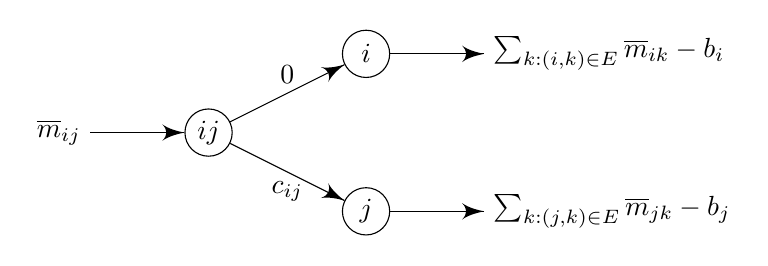
\begin{tikzpicture}
      \node [draw, circle, inner sep=0, minimum width=0.6cm] (ij) at (0, 0) {$ij$};
      \node [draw, circle, inner sep=0, minimum width=0.6cm] (i) at (2, 1) {$i$};
      \node [draw, circle, inner sep=0, minimum width=0.6cm] (j) at (2, -1) {$j$};
      \draw [->] (ij) -- (i) node [pos=0.5, above] {$0$};
      \draw [->] (ij) -- (j) node [pos=0.5, below] {$c_{ij}$};
      \draw [->] (-1.5, 0) node [left] {$\overline{m}_{ij}$} -- (ij);
      \draw [->] (i) -- +(1.5, 0) node [right] {$\sum_{k: (i, k)\in E}\overline{m}_{ik} - b_i$};
      \draw [->] (j) -- +(1.5, 0) node [right] {$\sum_{k: (j, k)\in E}\overline{m}_{jk} - b_j$};
    \end{tikzpicture}
  \end{center}
  The idea is that if the capacity of the edge $(i, j)$ is, say, 5, in the original network, and we want to transport $3$ along this edge, then in the new network, we send $3$ units from $ij$ to $j$, and $2$ units to $i$.

  The tricky part of the proof is to show that we have the same constraints in both graphs.

  For any flow $x$ in the original network, the corresponding flow on $(ij, j)$ is $x_{ij}$ and the flow on $(ij, i)$ is $\overline{m}_{ij} - x_{ij}$.  The total flow into $i$ is then
  \[
   \sum_{k: (i, j)\in E}(\overline{m}_{ik} - x_{ij}) + \sum_{k: (k, i)\in E}x_{ki}
  \]
  This satisfies the constraints of the new network if and only if
  \[
   \sum_{k: (i, j)\in E}(\overline{m}_{ik} - x_{ij}) + \sum_{k: (k, i)\in E}x_{ki} = \sum_{k: (i, k)\in E}\overline{m}_{ik} - b_i,
  \]
  which is true if and only if
  \[
    b_i + \sum_{k:(k, i)\in E}x_{ki} - \sum_{k: (i, k)\in E}x_{ik} = 0,
  \]
  which is exactly the constraint for the node $i$ in the original minimal-cost flow problem.
\end{proof}
To solve the transportation problem, it is convenient to have two sets of Lagrange multipliers, one for the supplier constraints and one for the consumer constraint. Then the Lagrangian of the transportation problem can be written as
\[
  L(x, \lambda, \mu) = \sum_{i = 1}^m\sum_{j = 1}^n c_{ij}x_{ij} + \sum_{i = 1}^n \lambda_i\left(s_i - \sum_{j = 1}^m x_{ij}\right) - \sum_{j = 1}^n \mu_j\left(d_j - \sum_{j = 1}^n x_{ij}\right).
\]
Note that we use different signs for the Lagrange multipliers for the suppliers and the consumers, so that our ultimate optimality condition will look nicer.

This is equivalent to
\[
  L(x, \lambda, \mu) = \sum_{i = 1}^n \sum_{j = 1}^n (c_{ij} - \lambda_i + \mu_j)x_{ij} + \sum_{i = 1}^n \lambda_i s_i - \sum_{j = 1}^m \mu_j d_j.
\]
Since is $x \geq 0$, the Lagrangian has a finite minimum iff $c_{ij} - \lambda_i + \mu_j \geq 0$ for all $i, j$. So this is our dual feasibility condition.

At an optimum, complementary slackness entails that
\[
  (c_{ij} - \lambda_i + \mu_j)x_{ij} = 0
\]
for all $i, j$.

In this case, we have a tableau as follows:
\newcommand\bb[1]{\multicolumn{1}{|c|}{#1}}
\newcommand\bbb[1]{\multicolumn{2}{c|}{#1}}
\newcommand\bbbb[1]{\multicolumn{2}{c}{#1}}
\begin{center}
  \begin{tabular}{c|cc|cc|cc|cc|c}
    \multicolumn{1}{c}{ } & \bbbb{$\mu_1$} & \bbbb{$\mu_2$} & \bbbb{$\mu_3$} & \bbbb{$\mu_4$}\\\cline{2-9}
    & \bbb{$\lambda_1 - \mu_1$} & \bbb{$\lambda_1 - \mu_2$} & \bbb{$\lambda_1 - \mu_3$} & \bbb{$\lambda_1 - \mu_4$}\\\cline{3-3}\cline{5-5}\cline{7-7}\cline{9-9}
    $\lambda_1$ & $x_{11}$ & \bb{$c_{11}$} & $x_{12}$ & \bb{$c_{12}$} & $x_{13}$ & \bb{$c_{13}$} & $x_{14}$ & \bb{$c_{14}$} & $s_1$\\\cline{2-9}
    & \bbb{$\lambda_2 - \mu_1$} & \bbb{$\lambda_2 - \mu_2$} & \bbb{$\lambda_2 - \mu_3$} & \bbb{$\lambda_2 - \mu_4$}\\\cline{3-3}\cline{5-5}\cline{7-7}\cline{9-9}
    $\lambda_2$ & $x_{21}$ & \bb{$c_{21}$} & $x_{22}$ & \bb{$c_{22}$} & $x_{23}$ & \bb{$c_{23}$} & $x_{24}$ & \bb{$c_{24}$} & $s_1$\\\cline{2-9}
    & \bbb{$\lambda_3 - \mu_1$} & \bbb{$\lambda_3 - \mu_2$} & \bbb{$\lambda_3 - \mu_3$} & \bbb{$\lambda_3 - \mu_4$}\\\cline{3-3}\cline{5-5}\cline{7-7}\cline{9-9}
    $\lambda_3$ & $x_{31}$ & \bb{$c_{31}$} & $x_{32}$ & \bb{$c_{32}$} & $x_{33}$ & \bb{$c_{33}$} & $x_{34}$ & \bb{$c_{34}$} & $s_1$\\\cline{2-9}
    \multicolumn{1}{c}{ }& \bbbb{$d_1$} & \bbbb{$d_2$} & \bbbb{$d_3$} & \bbbb{$d_4$}\\
  \end{tabular}
\end{center}
We have a row for each supplier and a column for each consumer.
\begin{eg}
  Suppose we have three suppliers with supplies $8, 10$ and $9$, and 4 consumers with demands $4, 5, 8, 8$.

  It is easy to create an initial feasible solution - we just start from the first consumer and first supplier, and supply as much as we can until one side runs out of stuff.

  We first fill our tableau with our feasible solution.
  \begin{center}
    \begin{tabular}{c|cc|cc|cc|cc|c}
      \cline{2-9}
      &   &        &   &        &   &        &   &        & \\\cline{3-3}\cline{5-5}\cline{7-7}\cline{9-9}
      & 6 & \bb{5} & 2 & \bb{3} &   & \bb{4} &   & \bb{6} & 8\\\cline{2-9}
      &   &        &   &        &   &        &   &        & \\\cline{3-3}\cline{5-5}\cline{7-7}\cline{9-9}
      &   & \bb{2} & 3 & \bb{7} & 7 & \bb{4} &   & \bb{1} & 10\\\cline{2-9}
      &   &        &   &        &   &        &   &        & \\\cline{3-3}\cline{5-5}\cline{7-7}\cline{9-9}
      &   & \bb{5} &   & \bb{6} & 1 & \bb{2} & 8 & \bb{4} & 9\\\cline{2-9}
      \multicolumn{1}{c}{ }& \bbbb{6}   & \bbbb{5} &\bbbb{8} & \bbbb{8} &
    \end{tabular}
  \end{center}
  \begin{center}
    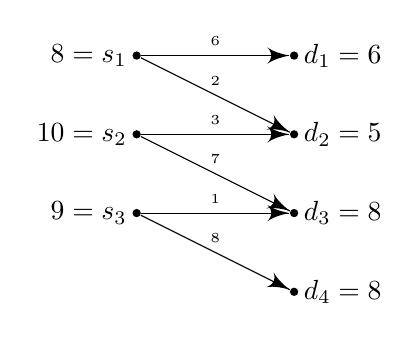
\begin{tikzpicture}
      \node (s1) at (0, 0) [circ] {};
      \node at (0, 0) [left] {$8 = s_1$};
      \node (s2) at (0, -1) [circ] {};
      \node at (0, -1) [left] {$10 = s_2$};
      \node (s3) at (0, -2) [circ] {};
      \node at (0, -2) [left] {$9 = s_3$};

      \node (d1) at (2, 0) [circ] {};
      \node at (2, 0) [right] {$d_1 = 6$};
      \node (d2) at (2, -1) [circ] {};
      \node at (2, -1) [right] {$d_2 = 5$};
      \node (d3) at (2, -2) [circ] {};
      \node at (2, -2) [right] {$d_3 = 8$};
      \node (d4) at (2, -3) [circ] {};
      \node at (2, -3) [right] {$d_4 = 8$};

      \draw [->] (s1) -- (d1) node [pos=0.5, above] {\tiny 6};
      \draw [->] (s1) -- (d2) node [pos=0.5, above] {\tiny 2};
      \draw [->] (s2) -- (d2) node [pos=0.5, above] {\tiny 3};
      \draw [->] (s2) -- (d3) node [pos=0.5, above] {\tiny 7};
      \draw [->] (s3) -- (d3) node [pos=0.5, above] {\tiny 1};
      \draw [->] (s3) -- (d4) node [pos=0.5, above] {\tiny 8};
    \end{tikzpicture}
  \end{center}
  We see that our basic feasible solution corresponds to a spanning tree. In general, if we have $n$ suppliers and $m$ consumers, then we have $n + m$ vertices, and hence $n + m - 1$ edges. So we have $n + m - 1$ dual constraints. So we can arbitrarily choose one Lagrange multiplier, and the other Lagrange multipliers will follow. We choose $\lambda_1 = 0$. Since we require
  \[
    (c_{ij} - \lambda_i + \mu_i)x_{ij} = 0,
  \]
  for edges in the spanning tree, $x_{ij} \not= 0$. So $c_{ij} - \lambda_i + \mu_i = 0$. Hence we must have $\mu_1 = -5$. We can fill in the values of the other Lagrange multipliers as follows, and obtain

  \begin{center}
    \begin{tabular}{c|cc|cc|cc|cc|}
      \multicolumn{1}{c}{ }& \bbbb{-5} & \bbbb{-3} & \bbbb{0} & \bbbb{-2}\\\cline{2-9}
      &   &        &   &        &   &        &   &       \\\cline{3-3}\cline{5-5}\cline{7-7}\cline{9-9}
      0 & 6 & \bb{5} & 2 & \bb{3} &   & \bb{4} &   & \bb{6}\\\cline{2-9}
      &   &        &   &        &   &        &   &       \\\cline{3-3}\cline{5-5}\cline{7-7}\cline{9-9}
      4 &   & \bb{2} & 3 & \bb{7} & 7 & \bb{4} &   & \bb{1}\\\cline{2-9}
      &   &        &   &        &   &        &   &       \\\cline{3-3}\cline{5-5}\cline{7-7}\cline{9-9}
      2 &   & \bb{5} &   & \bb{6} & 1 & \bb{2} & 8 & \bb{4}\\\cline{2-9}
    \end{tabular}
  \end{center}
  We can fill in the values of $\lambda_i - \mu_i$:
  \begin{center}
    \begin{tabular}{c|cc|cc|cc|cc|}
      \multicolumn{1}{c}{ }& \bbbb{-5} & \bbbb{-3} & \bbbb{0} & \bbbb{-2}\\\cline{2-9}
      &   &        &   &        & \bbb{0} & \bbb{2} \\\cline{3-3}\cline{5-5}\cline{7-7}\cline{9-9}
      0 & 6 & \bb{5} & 2 & \bb{3} &   & \bb{4} &   & \bb{6}\\\cline{2-9}
      & \bbb9       &   &        &   &        & \bbb{6}    \\\cline{3-3}\cline{5-5}\cline{7-7}\cline{9-9}
      4 &   & \bb{2} & 3 & \bb{7} & 7 & \bb{4} &   & \bb{1}\\\cline{2-9}
      & \bbb{7} & \bbb{5}  &   &        &   &       \\\cline{3-3}\cline{5-5}\cline{7-7}\cline{9-9}
      2 &   & \bb{5} &   & \bb{6} & 1 & \bb{2} & 8 & \bb{4}\\\cline{2-9}
    \end{tabular}
  \end{center}
  The dual feasibility condition is
  \[
    \lambda_i - \mu_i \leq c_{ij}
  \]
  If it is satisfied everywhere, we have optimality. Otherwise, will have to do something.

  What we do is add an edge, say from the second supplier to the second consumer. Then we have created a cycle. We keep increasing the flow on the new edge. This causes the values on other edges to change by flow conservation. So we keep doing this until some other edge reaches zero.

  If we increase flow by, say, $\delta$, we have
  \begin{center}
    \begin{tabular}{c|cc|cc|cc|cc|}
      \cline{2-9}
      &   &        &   &     &&&   &  \\\cline{3-3}\cline{5-5}\cline{7-7}\cline{9-9}
      & $6 - \delta$ & \bb{5} & $2 + \delta$ & \bb{3} &   & \bb{4} &   & \bb{6}\\\cline{2-9}
      &        &   &        &   & &&       &     \\\cline{3-3}\cline{5-5}\cline{7-7}\cline{9-9}
      & $\delta$ & \bb{2} & $3 - \delta$ & \bb{7} & 7 & \bb{4} &   & \bb{1}\\\cline{2-9}
      &  &   &   &        &   &    &  & \\\cline{3-3}\cline{5-5}\cline{7-7}\cline{9-9}
      &   & \bb{5} &   & \bb{6} & 1 & \bb{2} & 8 & \bb{4}\\\cline{2-9}
    \end{tabular}
  \end{center}

  \begin{center}
    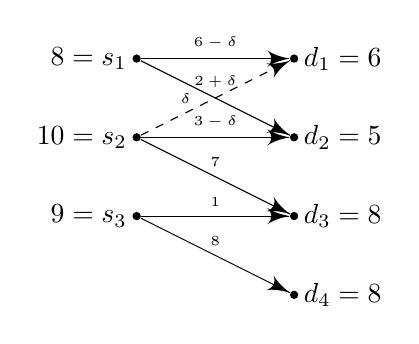
\begin{tikzpicture}
      \node (s1) at (0, 0) [circ] {};
      \node at (0, 0) [left] {$8 = s_1$};
      \node (s2) at (0, -1) [circ] {};
      \node at (0, -1) [left] {$10 = s_2$};
      \node (s3) at (0, -2) [circ] {};
      \node at (0, -2) [left] {$9 = s_3$};

      \node (d1) at (2, 0) [circ] {};
      \node at (2, 0) [right] {$d_1 = 6$};
      \node (d2) at (2, -1) [circ] {};
      \node at (2, -1) [right] {$d_2 = 5$};
      \node (d3) at (2, -2) [circ] {};
      \node at (2, -2) [right] {$d_3 = 8$};
      \node (d4) at (2, -3) [circ] {};
      \node at (2, -3) [right] {$d_4 = 8$};

      \draw [->] (s1) -- (d1) node [pos=0.5, above] {\tiny $6 - \delta$};
      \draw [->] (s1) -- (d2) node [pos=0.5, above] {\tiny $2 + \delta$};
      \draw [->] (s2) -- (d2) node [pos=0.5, above] {\tiny $3 - \delta$};
      \draw [->] (s2) -- (d3) node [pos=0.5, above] {\tiny 7};
      \draw [->] (s3) -- (d3) node [pos=0.5, above] {\tiny 1};
      \draw [->] (s3) -- (d4) node [pos=0.5, above] {\tiny 8};
      \draw [dashed, ->] (s2) -- (d1) node [pos=0.3, above] {\tiny $\delta$};
    \end{tikzpicture}
  \end{center}


  The maximum value of $\delta$ we can take is $3$. So we end up with

  \begin{center}
    \begin{tabular}{c|cc|cc|cc|cc|}
      \cline{2-9}
      &      &   &     &    &    & &&   \\\cline{3-3}\cline{5-5}\cline{7-7}\cline{9-9}
       & 3 & \bb{5} & 5 & \bb{3} &   & \bb{4} &   & \bb{6}\\\cline{2-9}
      &   &        & &      &   &        &  & \\\cline{3-3}\cline{5-5}\cline{7-7}\cline{9-9}
       & 3 & \bb{2} &  & \bb{7} & 7 & \bb{4} &   & \bb{1}\\\cline{2-9}
      & &       &         &    &    & & &\\\cline{3-3}\cline{5-5}\cline{7-7}\cline{9-9}
       &   & \bb{5} &   & \bb{6} & 1 & \bb{2} & 8 & \bb{4}\\\cline{2-9}
    \end{tabular}
  \end{center}

  We re-compute the Lagrange multipliers to obtain
  \begin{center}
    \begin{tabular}{c|cc|cc|cc|cc|}
      \multicolumn{1}{c}{ }& \bbbb{-5} & \bbbb{-3} & \bbbb{-7} & \bbbb{-9}\\\cline{2-9}
      &      &   &     &    & \bbb7   &  \bbb9  \\\cline{3-3}\cline{5-5}\cline{7-7}\cline{9-9}
      0 & 3 & \bb{5} & 5 & \bb{3} &   & \bb{4} &   & \bb{6}\\\cline{2-9}
      &   &        & \bbb0      &   &        &  \bbb9 \\\cline{3-3}\cline{5-5}\cline{7-7}\cline{9-9}
      -3 & 3 & \bb{2} &  & \bb{7} & 7 & \bb{4} &   & \bb{1}\\\cline{2-9}
      & \bbb0       & \bbb{-2}        &    &    & & \\\cline{3-3}\cline{5-5}\cline{7-7}\cline{9-9}
      -5 &   & \bb{5} &   & \bb{6} & 1 & \bb{2} & 8 & \bb{4}\\\cline{2-9}
    \end{tabular}
  \end{center}

  We see a violation at the bottom right. So we do it again:

  \begin{center}
    \begin{tabular}{c|cc|cc|cc|cc|}
      \cline{2-9}
      &      &   &     &    & &   &  &  \\\cline{3-3}\cline{5-5}\cline{7-7}\cline{9-9}
      & 3 & \bb{5} & 5 & \bb{3} &   & \bb{4} &   & \bb{6}\\\cline{2-9}
      &   &        & &      &   &        &  & \\\cline{3-3}\cline{5-5}\cline{7-7}\cline{9-9}
      & 3 & \bb{2} &  & \bb{7} & $7 - \delta$ & \bb{4} & $\delta$ & \bb{1}\\\cline{2-9}
      &     &   & &&        &    &    & \\\cline{3-3}\cline{5-5}\cline{7-7}\cline{9-9}
      &   & \bb{5} &   & \bb{6} & $1 + \delta$ & \bb{2} & $8 - \delta$ & \bb{4}\\\cline{2-9}
    \end{tabular}
  \end{center}

  The maximum possible value of $\delta$ is 7. So we have
  \begin{center}
    \begin{tabular}{c|cc|cc|cc|cc|}
      \cline{2-9}
      &      &   &     &    & &   &  &  \\\cline{3-3}\cline{5-5}\cline{7-7}\cline{9-9}
      & 3 & \bb{5} & 5 & \bb{3} &   & \bb{4} &   & \bb{6}\\\cline{2-9}
      &   &        & &      &   &     &  & \\\cline{3-3}\cline{5-5}\cline{7-7}\cline{9-9}
      & 3 & \bb{2} &  & \bb{7} &  & \bb{4} & 7 & \bb{1}\\\cline{2-9}
      & & & &      &    &  &  & \\\cline{3-3}\cline{5-5}\cline{7-7}\cline{9-9}
      &   & \bb{5} &   & \bb{6} & 8 & \bb{2} & 1 & \bb{4}\\\cline{2-9}
    \end{tabular}
  \end{center}

  Calculating the Lagrange multipliers gives
  \begin{center}
    \begin{tabular}{c|cc|cc|cc|cc|}
      \multicolumn{1}{c}{}& \bbbb{-5} & \bbbb{-3} & \bbbb{-2} & \bbbb{-4} \\\cline{2-9}
      &      &   &     &    & \bbb2   &  \bbb4  \\\cline{3-3}\cline{5-5}\cline{7-7}\cline{9-9}
      0 & 3 & \bb{5} & 5 & \bb{3} &   & \bb{4} &   & \bb{6}\\\cline{2-9}
      &   &        & \bbb0      &   \bbb{-1}     &  & \\\cline{3-3}\cline{5-5}\cline{7-7}\cline{9-9}
      -3 & 3 & \bb{2} &  & \bb{7} &  & \bb{4} & 7 & \bb{1}\\\cline{2-9}
      & \bbb{5} & \bbb{3}      &    &  &  & \\\cline{3-3}\cline{5-5}\cline{7-7}\cline{9-9}
      0 &   & \bb{5} &   & \bb{6} & 8 & \bb{2} & 1 & \bb{4}\\\cline{2-9}
    \end{tabular}
  \end{center}
  No more violations. Finally. So this is the optimal solution.
\end{eg}

\subsection{The maximum flow problem}
Suppose we have a network $(V, E)$ with a single source $1$ and a single sink $n$. There is no costs in transportation, but each edge has a capacity. We want to transport as much stuff from $1$ to $n$ as possible.

We can turn this into a minimum-cost flow problem. We add an edge from $n$ to $1$ with $-1$ cost and infinite capacity. Then the minimal cost flow will maximize the flow from $n$ to $1$ as possible. So the same amount of stuff will have to flow from $1$ to $n$ through the network.

We can write this is problem as
\begin{center}
  maximize $\delta$ subject to
  \[
    \sum_{j: (i, j) \in E}x_{ij} - \sum_{j(j, i)\in E}x_{ji} =
    \begin{cases}
      \delta & i = 1\\
      -\delta & i = n\\
      0&\text{otherwise}
    \end{cases}\quad\text{ for each }i
  \]
  \[
    0 \leq x_{ij}\leq C_{ij}\quad \text{ for each }(i, j)\in E.
  \]
\end{center}

However, we don't have to turn it into a minimum-cost flow problem. There are easier ways to solve the problem, using the \emph{max-flow min-cut theorem}.

\subsubsection{The max-flow min-cut theorem}

\begin{defi}[Cut]
  Suppose $G = (V, E)$ with capacities $C_{ij}$ for $(i, j)\in E$. A \emph{cut} of $G$ is a partition of $V$ into two sets.

  For $S\subseteq V$, the \emph{capacity} of the cut $(S, V\setminus S)$ is
  \[
    C(S) = \sum_{(i, j)\in (S\times (V\setminus S))\cap E}C_{ij},
  \]
  ie. the total capacity of the edges ``cut apart'' by the cut.
\end{defi}

Assume $x$ is a feasible flow vector that sends $\delta$ units from $1$ to $n$. For $X, Y\subseteq V$, we define
\[
  f_x(X, Y) = \sum_{(i, j)\in (X\times Y)\cap E}x_{ij},
\]
ie. the overall amount of flow from $X$ to $Y$.

Then for any cut $S\subseteq V$ with $1\in S, n\in V\setminus S$, we claim that
\[
  \delta = \sum_{i\in S}\left(\sum_{j: (i, j)\in E}x_{ij} - \sum_{j: (j, i)\in E}x_{ji}\right).
\]
This is true since by flow conservation, for any $i \not= 1$, $\sum_{j: (i, j) \in E}x_{ij} - \sum_{j: (j, i)\in E} = 0$, and for $i = 1$, it is $\delta$. So the sum is $\delta$. Hence
\begin{align*}
  \delta &= f_x(S, V) - f_x(V, S)\\
  &= f_x(S, S) + f_x(S, V\setminus S) - f_x(V\setminus S, S) - f_x(S, S)\\
  &= f_x(S, V\setminus S) - f_x(V\setminus S, S)\\
  &\leq f_x(S, V\setminus S)\\
  &\leq C(S)
\end{align*}
This says that the flow through the cut is less than the capacity through the cut, which is obviously true.

\begin{thm}[Max-flow min-cut theorem]
  Let $\delta$ be an optimal solution. Then
  \[
    \delta = \min\{C(S): S\subseteq V, 1\in S, n \in V\setminus S\}
  \]
\end{thm}

\begin{proof}
  Consider any feasible flow vector $x$. Call a path $v_0, \cdots, v_k$ an \emph{augmenting path} if the flow along the path can be increased. Formally, it is a path that satisfies
  \[
    x_{v_{i - 1}v_i} < C_{v_{i - 1}v_i}\text{ or }x_{v_iv_{i - 1}} > 0
  \]
  for $i = 1,\cdots, k$. The first condition says that we have a forward edge where we have not hit the capacity, while the second condition says that we have a backwards edge with positive flow. If these conditions are satisfied, we can increase the flow of each edge (or decrease the backwards flow for backwards edge), and the total flow increases.

  Now assume that $x$ is optimal and let
  \[
    S = \{1\}\cup \{i\in V: \text{ there exists an augmenting path from $1$ to $i$}\}.
  \]
  Since there is an augmenting path from $1$ to $S$, we can increase flow from $1$ to any vertex in $S$. So $n \not\in S$ by optimality. So $n\in V\setminus S$.

  We have previously shown that
  \[
    \delta = f_x(S, V\setminus S) - f_x(V\setminus S, S).
  \]
  We now claim that $f_x(V\setminus S, S) = 0$. If it is not $0$, it means that there is a node $v\in V\setminus S$ such that there is flow from $v$ to a vertex $u\in S$. Then we can add that edge to the augmenting path to $u$ to obtain an augmenting path to $v$.

  Also, we must have $f_x(S, V\setminus S) = C(S)$. Or else, we can still send more things to the other side so there is an augmenting path. So we have
  \[
    \delta = C(S).
  \]
\end{proof}

\subsubsection{Ford-Fulkerson algorithm}
The algorithm is simple:
\begin{enumerate}
  \item Start from a feasible flow $x$, eg. $x = \mathbf{0}$.
  \item If there is no augmenting path for $x$ form $1$ to $n$, then $x$ is optimal.
  \item Find an augmenting path for $x$ from $1$ to $n$, and send a maximum amount of flow along it. Go to 2.
\end{enumerate}

The max-flow min-cut theorem plays a role in step (ii). We can immediately prove that it is maximal by finding an appropriate cut.

\begin{eg}
  Consider the diagram
  \begin{center}
    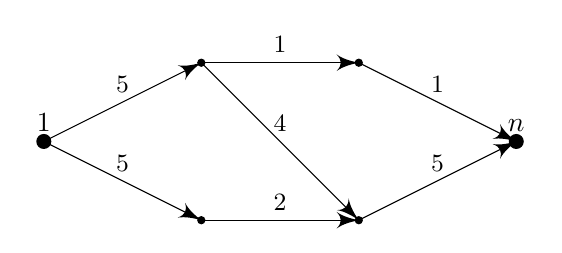
\begin{tikzpicture}[xscale=2]
      \node at (0, 0) [circ] {-};
      \node at (3, 0) [circ] {-};
      \node at (0, 0) [above] {1};
      \node at (3, 0) [above] {$n$};
      \draw [->] (0, 0) -- (1, 1) node [pos = 0.5, above] {\small 5};
      \draw [->] (1, 1) -- (2, 1) node [pos = 0.5, above] {\small 1};
      \draw [->] (2, 1) -- (3, 0) node [pos = 0.5, above] {\small 1};
      \draw [->] (0, 0) -- (1, -1) node [pos = 0.5, above] {\small 5};
      \draw [->] (1, -1) -- (2, -1) node [pos = 0.5, above] {\small 2};
      \draw [->] (2, -1) -- (3, 0) node [pos = 0.5, above] {\small 5};
      \draw [->] (1, 1) -- (2, -1) node [pos = 0.5, above] {\small 4};

      \node at (1, 1) [circ] {};
      \node at (2, 1) [circ] {};
      \node at (1, -1) [circ] {};
      \node at (2, -1) [circ] {};
    \end{tikzpicture}
  \end{center}
  We can keep adding flow until we reach
  \begin{center}
    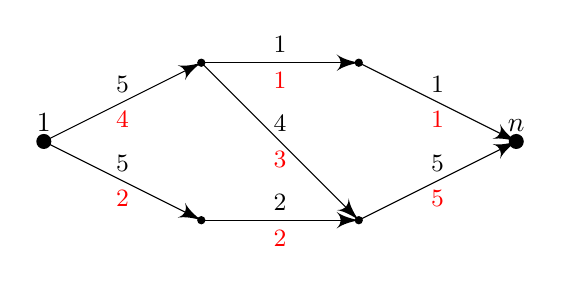
\begin{tikzpicture}[xscale=2]
      \node at (0, 0) [circ] {-};
      \node at (3, 0) [circ] {-};
      \node at (0, 0) [above] {1};
      \node at (3, 0) [above] {$n$};
      \draw [->] (0, 0) -- (1, 1) node [pos = 0.5, above] {\small 5};
      \draw [->] (1, 1) -- (2, 1) node [pos = 0.5, above] {\small 1};
      \draw [->] (2, 1) -- (3, 0) node [pos = 0.5, above] {\small 1};
      \draw [->] (0, 0) -- (1, -1) node [pos = 0.5, above] {\small 5};
      \draw [->] (1, -1) -- (2, -1) node [pos = 0.5, above] {\small 2};
      \draw [->] (2, -1) -- (3, 0) node [pos = 0.5, above] {\small 5};
      \draw [->] (1, 1) -- (2, -1) node [pos = 0.5, above] {\small 4};

      \node [red] at (0.5, 0.5) [below] {\small 4};
      \node [red] at (1.5, 1) [below] {\small 1};
      \node [red] at (2.5, 0.5) [below] {\small 1};
      \node [red] at (0.5, -0.5) [below] {\small 2};
      \node [red] at (1.5, -1) [below] {\small 2};
      \node [red] at (2.5, -0.5) [below] {\small 5};
      \node [red] at (1.5, 0) [below] {\small 3};

      \node at (1, 1) [circ] {};
      \node at (2, 1) [circ] {};
      \node at (1, -1) [circ] {};
      \node at (2, -1) [circ] {};
    \end{tikzpicture}
  \end{center}
  (red is flow, black is capacity). We know this is an optimum, since our total flow is $6$, and we can draw a cut with capacity 6:
  \begin{center}
    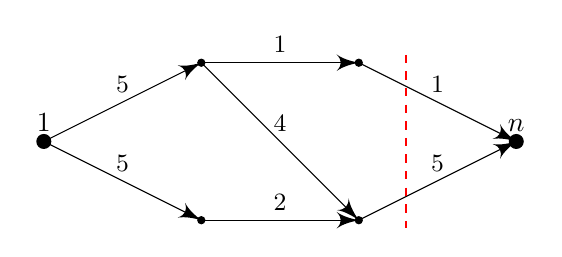
\begin{tikzpicture}[xscale=2]
      \node at (0, 0) [circ] {-};
      \node at (3, 0) [circ] {-};
      \node at (0, 0) [above] {1};
      \node at (3, 0) [above] {$n$};
      \draw [->] (0, 0) -- (1, 1) node [pos = 0.5, above] {\small 5};
      \draw [->] (1, 1) -- (2, 1) node [pos = 0.5, above] {\small 1};
      \draw [->] (2, 1) -- (3, 0) node [pos = 0.5, above] {\small 1};
      \draw [->] (0, 0) -- (1, -1) node [pos = 0.5, above] {\small 5};
      \draw [->] (1, -1) -- (2, -1) node [pos = 0.5, above] {\small 2};
      \draw [->] (2, -1) -- (3, 0) node [pos = 0.5, above] {\small 5};
      \draw [->] (1, 1) -- (2, -1) node [pos = 0.5, above] {\small 4};
      \draw [dashed, red] (2.3, 1.1) -- (2.3, -1.1);

      \node at (1, 1) [circ] {};
      \node at (2, 1) [circ] {};
      \node at (1, -1) [circ] {};
      \node at (2, -1) [circ] {};
    \end{tikzpicture}
  \end{center}
\end{eg}
\end{document}
